
\documentclass[12pt,openany]{book}

\setcounter{tocdepth}{1}
\setcounter{secnumdepth}{2}
% % % % % % % % % % % % % % % % % % % % % % % % % % % % % % % % % % % % %
%                       Paquetes y librerias                            %
% % % % % % % % % % % % % % % % % % % % % % % % % % % % % % % % % % % % %
\usepackage[utf8]{inputenc}
\usepackage[T1]{fontenc}
\usepackage{amsmath,amsfonts,amssymb,amsthm,latexsym,mathrsfs,color,graphicx}
\usepackage[english,spanish,es-noquoting]{babel}
\addto\captionsspanish{\renewcommand{\tablename}{Tabla}}
\usepackage{geometry}
\usepackage{graphicx}
\usepackage{epstopdf}
\usepackage{changepage}
\usepackage{float}
\usepackage{tabularx}
\usepackage{amsthm} 
\usepackage{longtable}
\usepackage{booktabs}

% Tablas apéndice
\usepackage{multirow}
\usepackage{pdflscape}
\usepackage{booktabs}



\usepackage{url}

\usepackage[hidelinks]{hyperref}

\usepackage[fixlanguage]{babelbib}
    \bibliographystyle{plain}
\usepackage{url} % necesario para \url{...} en el .bib


%\geometry{bindingoffset=2cm}
%\geometry{textwidth=390pt}
 \geometry{ a4paper, left=3cm, right=3cm, top=3cm,bottom=3cm}
\raggedbottom



% % % % % % % % % % % % % % % % % % % % % % % % % % % % % % % % % % % % %
%    Definicion de entornos y numeracion de teoremas, definiciones...   %
% % % % % % % % % % % % % % % % % % % % % % % % % % % % % % % % % % % % %
\theoremstyle{plain}
\newtheorem{theorem}{Teorema}[chapter]
\newtheorem{teor}[theorem]{Teorema}
\newtheorem{proposition}[theorem]{Proposición}
\newtheorem{lemma}[theorem]{Lema}
\newtheorem{corollary}[theorem]{Corolario}

\theoremstyle{definition}
\newtheorem{definition}{Definición}[chapter]
\newtheorem{example}{Ejemplo}[chapter]
\newtheorem{observation}{Observación}[chapter]
%\newtheorem{prop}[teor]{Proposición} % al ponerlo así considera que el contador es comun para los teoremas y las proposiciones

%\theoremstyle{remark}


% Declaracion de operadores
%\DeclareMathOperator{\dive}{\textrm{div}}

% Decimal con punto
\spanishdecimal{.}




% % % % % % % % % % % % % % % % % % % % % % % % % % % % % % % % % % % % %
%                               Portada                                 %
% % % % % % % % % % % % % % % % % % % % % % % % % % % % % % % % % % % % %
%     Los datos de la portada se cubren en el cuerpo del documento      %
%     como argumentos del comando \portada descrito a continuacion      %
% % % % % % % % % % % % % % % % % % % % % % % % % % % % % % % % % % % % %
\newcommand{\portada}[7]{
%\newcommand{\portada}[4]{
\thispagestyle{empty}

\vspace*{-2cm}
\begin{center}
\begin{minipage}{6cm}
		
\includegraphics[width=5cm]{logo_m2i}
	\end{minipage}\hspace{0.2cm}	
\end{center}
\begin{adjustwidth}{-2.5cm}{-2.5cm}
    \begin{minipage}{2.5cm}
    \vspace{0.5cm}		
    
\includegraphics[width=2cm]{logo_ux}
	\end{minipage} \hspace{0.2cm}
	\begin{minipage}{3.92cm}
		\vspace{0.5cm}
		
\includegraphics[width=3.92cm]{logo_udc}
	\end{minipage}\hspace{0.2cm}
	\begin{minipage}{3.52cm}
		\vspace{0.8cm}
		
\includegraphics[width=3.52cm]{logo_uvigo}
	\end{minipage}\hspace{0.2cm}
	\begin{minipage}{4.3cm}
		\vspace{0.15cm}
		
\includegraphics[width=4.3cm]{logo_UC3M}
	\end{minipage}\hspace{0.2cm}
	\begin{minipage}{2.22cm}
		\vspace{-0.5275cm}
		
\includegraphics[width=2.22cm]{logo_UPM}
	\end{minipage}
\end{adjustwidth}


\vspace{0.9cm}
\begin{center}
\bf
Máster en Matemática Industrial

\vspace{0.3cm}
Curso -- 2025-26

\vspace{2.3cm}
\large Proyecto Fin de Máster


\vspace{0.9cm}
{\Huge{\textbf{ #1 }}
\par}

\vspace{1.8cm}
{\Large #2 }
\end{center}


\vspace{4.8cm}
\noindent\begin{minipage}{\textwidth}
\begin{tabularx}{\textwidth}{@{}lX@{}}
\textbf{Fecha de presentación:} &  #6 \\
\textbf{Tutor académico:}&  #3\\
\textbf{Empresa:} & #4  \\%[0.5cm]
\textbf{Tutor de empresa: }& #7 \\
& \includegraphics[width=0.45\textwidth]{#5}
\end{tabularx}
\end{minipage}

\enlargethispage{5cm} {\pagestyle{empty}\cleardoublepage }}


% % % % % % % % % % % % % % % % % % % % % % % % % % % % % % % % % % % % %
%                               Resumen                                 %
% % % % % % % % % % % % % % % % % % % % % % % % % % % % % % % % % % % % %
% La ruta del fichero que contiene el resumen se cubre en el cuerpo del %
%documento como argumentos del comando \resumen descrito a continuacion %
% % % % % % % % % % % % % % % % % % % % % % % % % % % % % % % % % % % % %
\newcommand{\resumen}[1]{

\vspace*{3cm}
\noindent {\LARGE\bfseries Resumen}\par
\vspace*{2cm}

\input{#1}

\cleardoublepage }



% % % % % % % % % % % % % % % % % % % % % % % % % % % % % % % % % % % % %
% % % % % % % % % % % % % % % % % % % % % % % % % % % % % % % % % % % % %
% %                   Comienzo del documento                          % %
% % % % % % % % % % % % % % % % % % % % % % % % % % % % % % % % % % % % %
% % % % % % % % % % % % % % % % % % % % % % % % % % % % % % % % % % % % %
\begin{document}
\frontmatter


% % % % % % % % % % % % % % % % % % % % % % % % % % % % % % % % % % % % %
%                             Portada                                   %
% % % % % % % % % % % % % % % % % % % % % % % % % % % % % % % % % % % % %
\hypersetup{pageanchor=false}
\portada{Entropía Relativa versus Volatilidad Local Estocástica:\\[0.1cm]
{\Large Comparación de las dos estrategias dinámicas de cobertura.}}{Miriam Gutiérrez Serrano}{Carlos Vázquez Cendón (UDC)}{Banco Santander}{Banco_Santander_Logotipo.png}{Julio 2026}{Daniel Arrieta Rodríguez y Cristina Arribas Francisco}
\hypersetup{pageanchor=true}



% Reinicio del contador de paginas
\setcounter{page}{1}

% % % % % % % % % % % % % % % % % % % % % % % % % % % % % % % % % % % % %
%                             Indice                                    %
% % % % % % % % % % % % % % % % % % % % % % % % % % % % % % % % % % % % %
\tableofcontents

\cleardoublepage


% % % % % % % % % % % % % % % % % % % % % % % % % % % % % % % % % % % % %
%                             Resumen                                   %
% % % % % % % % % % % % % % % % % % % % % % % % % % % % % % % % % % % % %
\addcontentsline{toc}{chapter}{Resumen}
\markboth{Resumen}{ }
\resumen{resumen.tex}
% El argumento debe incluir la ruta del .tex del resumen


% % % % % % % % % % % % % % % % % % % % % % % % % % % % % % % % % % % % %
%                       Cuerpo del documento                            %
% % % % % % % % % % % % % % % % % % % % % % % % % % % % % % % % % % % % %
\mainmatter


\chapter{Introducción}

En los mercados financieros actuales, la correcta valoración de productos derivados es un elemento clave tanto para la gestión del riesgo como para la toma de decisiones. La complejidad observada en las superficies de volatilidad implícita hace necesario el uso de modelos capaces de reproducir con precisión las dinámicas de mercado, especialmente en contextos en los que los supuestos clásicos resultan insuficientes. \medskip

Aunque los instrumentos derivados se negocian desde mucho antes de la formalización matemática moderna, el desarrollo sistemático de modelos de valoración comenzó a consolidarse a mediados del siglo XX, cuando la combinación de procesos estocásticos, cálculo de Itô y argumentos de ausencia de arbitraje permitió construir un marco riguroso para obtener precios consistentes con el mercado. \medskip

Un punto de inflexión en esta evolución fue la publicación, en 1973, del modelo de Black--Scholes para la valoración de opciones europeas, posteriormente ampliado por Merton. Este modelo proporcionó una fórmula cerrada para el precio de opciones bajo hipótesis muy concretas, entre ellas que el precio del activo subyacente sigue una dinámica lognormal con volatilidad constante.  \medskip

Sin embargo, con el paso del tiempo se observó que algunas de las hipótesis del modelo no se ajustaban completamente al comportamiento real de los mercados. En particular, la volatilidad implícita obtenida a partir de los precios observados no era constante, sino que dependía tanto del strike como del vencimiento de la opción. Este fenómeno, conocido como smile o superficie de volatilidad, se hizo especialmente relevante tras el desplome bursátil del 19 de octubre de 1987, conocido como Black Monday, al poner de manifiesto que los mercados asignaban una mayor probabilidad a movimientos extremos de la que implicaba el modelo lognormal clásico. \medskip

La aparición de la superficie de volatilidad motivó el desarrollo de modelos capaces de reproducir de forma más precisa los precios de mercado. En esta memoria nos centraremos en el estudio de dos metodologías que permiten abordar esta cuestión desde enfoques diferentes.

Por un lado, los modelos de Volatilidad Local Estocástica surgen como un enfoque híbrido que combina las ventajas de los modelos de volatilidad local y de volatilidad estocástica, permitiendo un ajuste preciso a las cotizaciones observadas en el mercado y una representación más realista de la evolución futura de la volatilidad.

Por otro lado, el enfoque basado en Entropía Relativa Mínima proporciona un marco general de calibración y valoración en mercados incompletos, en el que se selecciona la medida de valoración más cercana a una medida previa, sujeta a la imposición de restricciones de mercado. En la práctica, emplearemos el método de Weighted Monte Carlo, que permite incorporar información de mercado modificando las probabilidades asociadas a la simulación original. \medskip

El objetivo principal de este trabajo es analizar y comparar ambos enfoques desde un punto de vista teórico y práctico, identificando sus principales ventajas, limitaciones y ámbitos de aplicación.

En primer lugar, abordaremos el marco teórico necesario para el desarrollo del trabajo, que incluye los fundamentos de los procesos estocásticos aplicados a la modelización financiera, la dinámica de los precios de los activos bajo medidas de probabilidad equivalentes y los principios básicos de valoración de derivados financieros. Asimismo, presentaremos el modelo de Black--Scholes y sus principales limitaciones, con el fin de motivar el estudio de los nuevos métodos. \medskip

En segundo lugar, estudiaremos en detalle el modelo de Volatilidad Local Estocástica, introduciendo previamente los modelos de volatilidad local y de volatilidad estocástica, así como su combinación en el marco SLV. Por otra parte, estudiaremos el enfoque de Entropía Relativa Mínima como método de calibración y valoración en mercados incompletos. En esta fase se analizará su formulación teórica, su interpretación probabilística como un problema de optimización bajo restricciones y su relación con el cambio de medida. \medskip

A partir de este análisis, se desarrollarán simulaciones numéricas con el fin de analizar el comportamiento de los modelos y su capacidad para reproducir las dinámicas observadas en los mercados. Por último, llevaremos a cabo una comparación sistemática entre los enfoques SLV y MRE, evaluando su comportamiento en el contexto de opciones europeas vainilla y opciones de tipo \textit{forward-start}. Este análisis permitirá estudiar las ventajas y limitaciones de cada metodología en un entorno de mayor complejidad, propio de productos exóticos.

\chapter[Conceptos preliminares y Black--Scholes]{Conceptos preliminares y modelo de Black--Scholes}

En este capítulo vamos a introducir los conceptos teóricos que serán necesarios a lo largo del trabajo. El objetivo es fijar el marco probabilístico y financiero común en el que ambos modelos se formulan. En particular, partiremos de las nociones básicas de mercado financiero, ausencia de arbitraje y valoración neutral al riesgo, para después presentar el modelo de Black--Scholes y explicar por qué sus hipótesis no son suficientes para reproducir los precios observados en mercado.\medskip

La notación utilizada seguirá principalmente \cite{DanielArrietaPresentation}. Para la formulación del modelo de Black--Scholes y la metodología de cobertura dinámica tomaremos como referencia \cite{CarlosVazquezMAT}. Asimismo, para la interpretación del cambio de medida, la valoración mediante esperanzas y la motivación de los modelos de volatilidad local estocástica se tendrá en cuenta \cite{oosterlee2021modelos}.\medskip

\section{Conceptos preliminares}

Consideramos un espacio de probabilidad filtrado
\[
(\Omega,\mathcal{F},\{\mathcal{F}_t\}_{t\geq 0},\mathbb{P}),
\]
donde \(\Omega\) representa el conjunto de posibles estados del mercado, \(\mathcal{F}\) es una \(\sigma\)-álgebra, \(\mathbb{P}\) es la medida de probabilidad real, y \(\{\mathcal{F}_t\}_{t\geq 0}\) es una filtración que recoge la información disponible hasta cada instante \(t\).

En este contexto, los precios de los activos financieros se modelan mediante procesos estocásticos adaptados a la filtración. Esto significa que, en cada instante de tiempo, el precio observado solo depende de la información disponible hasta ese momento. Una noción especialmente importante en valoración financiera es la de martingala. La siguiente noción será fundamental para formular la valoración sin arbitraje.

\begin{definition}
\label{def:martingala}
Un proceso estocástico \(\{X(t)\}_{t\geq 0}\) se dice martingala respecto de la filtración \(\{\mathcal{F}_t\}_{t\geq 0}\) y de la medida \(\mathbb{P}\) si es adaptado, integrable, y verifica
\[
\mathbb{E}^{\mathbb{P}}\left[X(T)\mid \mathcal{F}_t\right]=X(t),
\qquad t\leq T.
\]
\end{definition}

Intuitivamente, una martingala representa un proceso cuyo valor actual es la mejor predicción de su valor futuro, teniendo en cuenta la información disponible. En valoración financiera esta propiedad aparece de forma natural al estudiar precios descontados bajo una medida de probabilidad adecuada.

Consideramos ahora un mercado financiero formado por \(M+1\) activos. Denotaremos por
\[
S^{(0)}(t),S^{(1)}(t),\ldots,S^{(M)}(t)
\]
los procesos de precios correspondientes. El activo \(S^{(0)}(t)\) suele representar la cuenta bancaria libre de riesgo y se toma como numerario. Lo denotaremos por
\[
N(t):=S^{(0)}(t).
\]
El numerario permite expresar los precios en unidades relativas. Así, en lugar de estudiar directamente \(S^{(m)}(t)\), se consideran los precios descontados
\[
\frac{S^{(m)}(t)}{N(t)}, \qquad m=1,\ldots,M.
\]

Introducimos ahora las estrategias de inversión, que describen cómo se reparte la cartera entre los distintos activos del mercado.

\begin{definition}
\label{def:estrategia-inversion}
Una estrategia de inversión es una familia de procesos
\[
h(t)=\left(h^{(0)}(t),h^{(1)}(t),\ldots,h^{(M)}(t)\right),
\]
donde \(h^{(m)}(t)\) representa el número de unidades del activo \(S^{(m)}(t)\) mantenidas en cartera en el instante \(t\). El valor de la cartera viene dado por
\[
V(t)=h^{(0)}(t)S^{(0)}(t)+\sum_{m=1}^{M}h^{(m)}(t)S^{(m)}(t).
\]
Diremos que la cartera es autofinanciada si sus variaciones de valor proceden únicamente de los cambios en los precios de los activos que la componen, sin aportaciones ni retiradas externas de capital.
\end{definition}

La hipótesis fundamental sobre la que se construye la valoración de derivados es la ausencia de arbitraje. De forma intuitiva, una oportunidad de arbitraje es una estrategia que permite obtener un beneficio sin asumir riesgo y sin realizar una inversión inicial neta. La existencia de arbitraje indicaría una inconsistencia en los precios del mercado. Formalicemos esta idea mediante la siguiente definición.

\begin{definition}
\label{def:oportunidad-arbitraje}
Una oportunidad de arbitraje es una cartera autofinanciada que verifica alguna de las siguientes condiciones:
\[
V(0)<0,\qquad V(T)\geq 0,
\]
o bien
\[
V(0)=0,\qquad V(T)\geq 0,\qquad 
\mathbb{P}(V(T)>0)>0.
\]
\end{definition}

La primera situación representa un beneficio inicial sin coste futuro. La segunda describe una estrategia sin inversión inicial, sin posibilidad de pérdida y con probabilidad positiva de ganancia.

Los activos derivados se incorporan a este marco como contratos cuyo valor depende de uno o varios activos subyacentes.

\begin{definition}
\label{def:derivado}
Un derivado con vencimiento \(T\) es un contrato financiero cuyo pago final es una variable aleatoria \(H\), medible respecto de \(\mathcal{F}_T\). En muchos casos puede escribirse como
\[
H=g(S(T)),
\]
donde \(S(T)\) representa el valor del subyacente en el vencimiento.
\end{definition}

Por ejemplo, el payoff de una opción call europea con strike \(K\) es
\[
H=\max\{S(T)-K,0\},
\]
mientras que el payoff de una opción put europea es
\[
H=\max\{K-S(T),0\}.
\]

El siguiente resultado resume la relación entre ausencia de arbitraje y existencia de una medida de valoración.

\begin{theorem}[Primer Teorema Fundamental de Valoración Financiera]
\label{th:primer-teorema-fundamental}
Un mercado financiero está libre de arbitraje si y solo si existe una medida de probabilidad \(\mathbb{Q}\), equivalente a \(\mathbb{P}\), bajo la cual los precios expresados en unidades del numerario son martingalas. Es decir,
\[
\frac{S^{(m)}(t)}{N(t)}
=
\mathbb{E}^{\mathbb{Q}}\left[
\frac{S^{(m)}(T)}{N(T)}
\mid \mathcal{F}_t
\right],
\qquad m=1,\ldots,M,\quad t\leq T.
\]
\end{theorem}

La medida \(\mathbb{Q}\) se denomina medida martingala equivalente. Cuando el numerario es la cuenta bancaria libre de riesgo, esta medida recibe el nombre de medida neutral al riesgo.

Como consecuencia, si \(H\) es el pago de un derivado en el vencimiento \(T\), su precio en el instante \(t\) viene dado por
\[
V(t)
=
N(t)\,
\mathbb{E}^{\mathbb{Q}}\left[
\frac{H}{N(T)}
\mid \mathcal{F}_t
\right].
\]
En particular, si el tipo de interés libre de riesgo \(r\) es constante y el numerario es \(N(t)=e^{rt}\), entonces
\[
V(t)
=
e^{-r(T-t)}
\mathbb{E}^{\mathbb{Q}}\left[
H\mid \mathcal{F}_t
\right].
\]

Este resultado es fundamental porque permite interpretar la valoración de derivados como un problema de cálculo de esperanzas bajo una medida adecuada. Sin embargo, el teorema anterior no garantiza que dicha medida sea única. Para ello es necesario introducir la noción de mercado completo.

\begin{definition}
\label{def:derivado-replicable}
Un derivado con pago \(H\) se dice replicable si existe una cartera autofinanciada \(V\) tal que
\[
V(T)=H.
\]
Un mercado se dice completo si todo derivado puede ser replicado mediante una cartera autofinanciada.
\end{definition}

Así, la relación entre completitud del mercado y unicidad de la medida de valoración queda recogida en el siguiente resulDtado.

\begin{theorem}[Segundo Teorema Fundamental de Valoración Financiera]
\label{th:segundo-teorema-fundamental}
Supongamos que el mercado está libre de arbitraje. Entonces, el mercado es completo si y solo si existe una única medida martingala equivalente.
\end{theorem}

%REVISAR SI ES CIERTO CUANDO VICTOR TE PASE EL LIBRO SI LA DEMOSTRACIÓN ESTA EN EL LIBRO Y EN ESAS PÁGINAS
Una demostración de estos dos últimos resultados se pueden encontrar en \cite[pp.92--98]{Capinski2012}. \medskip

Por tanto, en un mercado completo, el precio de cualquier derivado replicable queda determinado de forma única por ausencia de arbitraje. En cambio, en un mercado incompleto pueden existir varias medidas martingala equivalentes y, en consecuencia, distintos precios compatibles con ausencia de arbitraje para un mismo derivado no replicable.

Para formalizar el paso de una medida de probabilidad a otra, introducimos primero la noción de continuidad absoluta.

\begin{definition}
\label{def:continuidad-absoluta}
Sean \((\Omega,\mathcal{F})\) un espacio medible y \(\mathbb{P}\), \(\mathbb{Q}\) dos medidas de probabilidad sobre dicho espacio. Diremos que \(\mathbb{Q}\) es absolutamente continua respecto de \(\mathbb{P}\), y escribiremos \(\mathbb{Q}\ll \mathbb{P}\), si para todo \(A\in\mathcal{F}\) se cumple que
\[
\mathbb{P}(A)=0, \quad \text{entonces} \quad \mathbb{Q}(A)=0.
\]
Si \(\mathbb{Q}\ll \mathbb{P}\) y \(\mathbb{P}\ll \mathbb{Q}\), diremos que ambas medidas son equivalentes.
\end{definition}

Si \(\mathbb{Q}\ll \mathbb{P}\), el teorema de Radon--Nikodym garantiza la existencia de una variable aleatoria no negativa, denotada por
\[
\frac{d\mathbb{Q}}{d\mathbb{P}},
\]
tal que, para todo \(A\in\mathcal{F}\),
\begin{equation}
\label{eq:radon-nikodym}
\mathbb{Q}(A)
=
\int_A \frac{d\mathbb{Q}}{d\mathbb{P}}\,d\mathbb{P}.
\end{equation}
A esta variable aleatoria se le denomina derivada de Radon--Nikodym de \(\mathbb{Q}\) respecto de \(\mathbb{P}\). Además, permite expresar esperanzas bajo la medida \(\mathbb{Q}\) en términos de esperanzas bajo la medida \(\mathbb{P}\). En particular, para una variable aleatoria integrable \(X\), se tiene
\[
\mathbb{E}^{\mathbb{Q}}[X]
=
\mathbb{E}^{\mathbb{P}}
\left[
X\frac{d\mathbb{Q}}{d\mathbb{P}}
\right].
\]

En el contexto de procesos estocásticos continuos, el resultado que describe cómo cambia la dinámica de un proceso al realizar un cambio de medida es el teorema de Cameron--Martin--Girsanov.

\begin{theorem}[Teorema de Cameron--Martin--Girsanov]
\label{th:girsanov}
Sea \(W(t)\) un movimiento browniano bajo la medida \(\mathbb{P}\), y sea \(\gamma(t)\) un proceso \(\mathcal{F}\)-previsible que satisface
\[
\mathbb{E}^{\mathbb{P}}
\left[
\exp\left(
\frac{1}{2}\int_0^T \gamma^2(t)\,dt
\right)
\right]
<\infty.
\]
Entonces existe una medida \(\mathbb{Q}\), equivalente a \(\mathbb{P}\), tal que
\[
\frac{d\mathbb{Q}}{d\mathbb{P}}
=
\exp\left(
-\int_0^T \gamma(t)\,dW(t)
-
\frac{1}{2}\int_0^T \gamma^2(t)\,dt
\right),
\]
y el proceso
\[
\widetilde{W}(t)
=
W(t)
+
\int_0^t \gamma(s)\,ds
\]
es un movimiento browniano bajo \(\mathbb{Q}\).
\end{theorem}

El teorema anterior muestra que un cambio de medida permite transformar un movimiento browniano bajo \(\mathbb{P}\) en un movimiento browniano bajo \(\mathbb{Q}\), incorporando un término de deriva. Esta idea resulta fundamental en valoración financiera, ya que permite pasar de una medida real o histórica a una medida neutral al riesgo.

Para verlo de forma más explícita, supongamos que \(X\) es un proceso de Itô dado por
\[
dX(t)
=
\mu(t)\,dt+\sigma(t)\,dW(t),
\]
donde \(W\) es un movimiento browniano bajo \(\mathbb{P}\). Supongamos que queremos encontrar una medida \(\mathbb{Q}\) bajo la cual la deriva del proceso sea \(\nu(t)\,dt\) en lugar de \(\mu(t)\,dt\). Entonces podemos reescribir
\[
dX(t)
=
\sigma(t)
\left(
dW(t)
+
\frac{\mu(t)-\nu(t)}{\sigma(t)}\,dt
\right)
+
\nu(t)\,dt.
\]
Si definimos
\[
\gamma(t)
:=
\frac{\mu(t)-\nu(t)}{\sigma(t)},
\]
y si \(\gamma\) satisface la condición de integrabilidad del teorema de Cameron--Martin--Girsanov, entonces existe una medida \(\mathbb{Q}\) tal que
\[
\widetilde{W}(t)
=
W(t)
+
\int_0^t
\frac{\mu(s)-\nu(s)}{\sigma(s)}\,ds
\]
es un movimiento browniano bajo \(\mathbb{Q}\). Por tanto, bajo la nueva medida, el proceso \(X\) puede escribirse como
\[
dX(t)
=
\nu(t)\,dt+\sigma(t)\,d\widetilde{W}(t).
\]

Esta discusión será importante en el desarrollo posterior del trabajo. Por una parte, justifica el paso de una medida real a una medida neutral al riesgo en modelos como Black--Scholes. Por otra parte, permite interpretar la metodología de Entropía Relativa Mínima como un procedimiento de selección de medida en un mercado incompleto. En este último caso, el cambio de medida no se construye modificando directamente la deriva de una ecuación diferencial estocástica, sino ajustando los pesos asignados a las trayectorias simuladas. Así, entre todas las medidas que reproducen determinadas restricciones de mercado, se escoge aquella que se mantiene más próxima a una medida previa.

El modelo de Black--Scholes constituye el ejemplo clásico en el que estas ideas se concretan de forma explícita. Bajo sus hipótesis, el mercado es completo y la medida neutral al riesgo es única, lo que permite obtener una fórmula cerrada para el precio de opciones europeas. Sin embargo, como veremos a continuación, sus supuestos también introducen limitaciones importantes que motivan el estudio de modelos más flexibles.

\section{El modelo de Black--Scholes y sus limitaciones}

El modelo de Black--Scholes constituye uno de los pilares de la valoración moderna de derivados. Su importancia no reside únicamente en la fórmula cerrada que proporciona para opciones europeas, sino también en la interpretación financiera basada en la cobertura dinámica. Bajo sus hipótesis, el precio de una opción se obtiene construyendo una cartera autofinanciada que replica exactamente el payoff final del derivado.

Consideramos un mercado formado por una cuenta bancaria libre de riesgo \(B(t)\) y un activo con riesgo \(S(t)\). La cuenta bancaria evoluciona según
\[
dB(t)=rB(t)\,dt,
\]
donde \(r\) es el tipo de interés libre de riesgo. Por otra parte, el activo subyacente sigue, bajo la medida \(\mathbb{P}\), la dinámica
\[
dS(t)=\mu S(t)\,dt+\sigma S(t)\,dW^{\mathbb{P}}(t),
\]
donde \(\mu\) es la rentabilidad esperada, \(\sigma>0\) es la volatilidad constante y \(W^{\mathbb{P}}(t)\) es un movimiento browniano bajo \(\mathbb{P}\).

Aplicando el lema de Itô a \(\log S(t)\), se obtiene
\[
S(t)
=
S_0
\exp\left[
\left(\mu-\frac{1}{2}\sigma^2\right)t
+
\sigma W^{\mathbb{P}}(t)
\right].
\]
Por tanto, el modelo supone que el precio del subyacente sigue una distribución lognormal.

Para valorar derivados, se trabaja bajo la medida neutral al riesgo \(\mathbb{Q}\). Bajo esta medida, el drift del subyacente deja de ser \(\mu\) y pasa a ser el tipo libre de riesgo \(r\). Así,
\[
dS(t)=rS(t)\,dt+\sigma S(t)\,dW^{\mathbb{Q}}(t).
\]
El cambio de medida modifica el término de tendencia, pero no elimina el papel central de la volatilidad. De hecho, la volatilidad es el parámetro que determina la dispersión de los posibles valores futuros del subyacente y, por tanto, influye de forma esencial en el precio de las opciones.

Sea \(V(S,t)\) el precio en el instante \(t\) de un derivado europeo con payoff
\[
V(S,T)=g(S).
\]
Bajo las hipótesis anteriores, el precio satisface la ecuación de Black--Scholes.

\begin{theorem}[Ecuación de Black--Scholes]
\label{th:ecuacion-black-scholes}
Supongamos que el precio del subyacente sigue, bajo la medida neutral al riesgo, la dinámica
\[
dS(t)=rS(t)\,dt+\sigma S(t)\,dW^{\mathbb{Q}}(t).
\]
Entonces el precio \(V(S,t)\) de un derivado europeo con condición final \(V(S,T)=g(S)\) satisface la ecuación
\[
\frac{\partial V}{\partial t}
+
rS\frac{\partial V}{\partial S}
+
\frac{1}{2}\sigma^2S^2
\frac{\partial^2 V}{\partial S^2}
-
rV
=0.
\]
\end{theorem}

Esta ecuación puede obtenerse mediante un argumento de cobertura dinámica. La idea consiste en construir una cartera formada por una posición en el derivado y una posición en el subyacente, escogida de forma que el término aleatorio desaparezca. Al eliminarse el riesgo instantáneo, la cartera debe crecer al tipo libre de riesgo, pues de lo contrario existiría una oportunidad de arbitraje.

De forma equivalente, la ecuación anterior puede interpretarse mediante el teorema de Feynman--Kac, que relaciona ciertas ecuaciones en derivadas parciales parabólicas con esperanzas condicionadas bajo una medida de probabilidad.

\begin{theorem}[Feynman--Kac]
\label{th:feynman-kac}
Sea \(X(t)\) un proceso que, bajo una medida \(\mathbb{Q}\), satisface
\[
dX(t)=a(X(t),t)\,dt+b(X(t),t)\,dW^{\mathbb{Q}}(t).
\]
Si \(V(X,t)\) es suficientemente regular y satisface
\[
\frac{\partial V}{\partial t}
+
a(X,t)\frac{\partial V}{\partial X}
+
\frac{1}{2}b^2(X,t)\frac{\partial^2 V}{\partial X^2}
-
r(X,t)V
=0,
\]
con condición final \(V(X(T),T)\), entonces
\[
V(X(t),t)
=
\mathbb{E}^{\mathbb{Q}}
\left[
\exp\left(-\int_t^T r(X(s),s)\,ds\right)
V(X(T),T)
\mid \mathcal{F}_t
\right].
\]
\end{theorem}

En el caso particular del modelo de Black--Scholes, se tiene
\[
a(S,t)=rS,
\qquad
b(S,t)=\sigma S.
\]
Por tanto, la valoración mediante ecuaciones en derivadas parciales y la valoración mediante esperanzas descontadas bajo \(\mathbb{Q}\) conducen al mismo precio.

Para una opción call europea con strike \(K\) y vencimiento \(T\), cuyo payoff es
\[
\max\{S(T)-K,0\},
\]
la solución de la ecuación de Black--Scholes viene dada por la conocida fórmula cerrada.

\begin{proposition}[Fórmula de Black--Scholes]
\label{prop:formula-black-scholes}
En el modelo de Black--Scholes, el precio en \(t=0\) de una opción call europea con strike \(K\), vencimiento \(T\), tipo de interés constante \(r\) y volatilidad constante \(\sigma\), es
\[
C_{BS}(S_0,K,T,r,\sigma)
=
S_0\Phi(d_1)
-
Ke^{-rT}\Phi(d_2),
\]
donde
\[
d_1=
\frac{
\log(S_0/K)+\left(r+\frac{1}{2}\sigma^2\right)T
}{
\sigma\sqrt{T}
},
\qquad
d_2=d_1-\sigma\sqrt{T},
\]
y \(\Phi\) denota la función de distribución de una normal estándar.
\end{proposition}

Análogamente, el precio de una opción put europea viene dado por
\[
P_{BS}(S_0,K,T,r,\sigma)
=
Ke^{-rT}\Phi(-d_2)
-
S_0\Phi(-d_1).
\]

El modelo de Black--Scholes es, por tanto, un modelo cerrado y coherente desde el punto de vista matemático. Sin embargo, sus hipótesis son demasiado restrictivas para reproducir de forma precisa los precios observados en mercado. En particular, el modelo supone que la volatilidad \(\sigma\) es constante, que el subyacente sigue una dinámica lognormal, que no hay costes de transacción, que la negociación es continua y que la cobertura puede realizarse de forma exacta.

En la práctica, estas hipótesis no se cumplen de forma exacta. Una de las evidencias más claras es la existencia de la volatilidad implícita. Dado un precio de mercado \(C^{mkt}(K,T)\), se define la volatilidad implícita como el valor \(\sigma_{imp}(K,T)\) que hace que la fórmula de Black--Scholes reproduzca dicho precio:
\[
C_{BS}(S_0,K,T,r,\sigma_{imp}(K,T))
=
C^{mkt}(K,T).
\]

\begin{definition}
\label{def:volatilidad-implicita}
La volatilidad implícita asociada a una opción de strike \(K\) y vencimiento \(T\) es el valor \(\sigma_{imp}(K,T)\) que, introducido en la fórmula de Black--Scholes, iguala el precio teórico al precio observado en mercado.
\end{definition}

Si el modelo de Black--Scholes describiese correctamente el mercado, la volatilidad implícita debería ser la misma para todos los strikes y vencimientos. Sin embargo, esto no ocurre en la práctica. Para un vencimiento fijo, la aplicación
\[
K\longmapsto \sigma_{imp}(K,T)
\]
no suele ser constante. Su representación gráfica recibe el nombre de sonrisa o \textit{skew} de volatilidad. Al considerar simultáneamente distintos vencimientos, se obtiene la superficie de volatilidad implícita:
\[
(K,T)\longmapsto \sigma_{imp}(K,T).
\]

La existencia de la superficie de volatilidad muestra que una única volatilidad constante no permite reproducir simultáneamente los precios de mercado para distintos strikes y vencimientos. Por tanto, aunque Black--Scholes proporciona un marco teórico coherente, la hipótesis de dinámica lognormal con volatilidad constante resulta demasiado restrictiva para capturar la información contenida en los precios observados.

En este contexto, la volatilidad implícita no debe interpretarse solo como un parámetro del modelo, sino como una forma de resumir la información de mercado. Su dependencia respecto del strike y del vencimiento evidencia la necesidad de introducir metodologías más flexibles.

Esta limitación motiva el estudio de los modelos de Volatilidad Local Estocástica, que enriquecen la dinámica del subyacente y de su volatilidad para ajustarse mejor a la superficie observada. Posteriormente, se introducirá la metodología de Entropía Relativa Mínima, que aborda el problema desde otra perspectiva: modificar la medida de probabilidad de los escenarios simulados para incorporar restricciones de mercado.\medskip

\subsection*{Opciones forward--start}
En la comparación numérica de ambos enfoques se considerarán tanto opciones vainilla europeas como opciones de tipo \textit{forward-start}, estas últimas especialmente útiles para analizar el comportamiento de cada metodología ante productos sensibles a la evolución futura de la volatilidad.

Una opción \textit{forward-start} es una opción cuyo periodo de referencia comienza en una fecha futura \(T_1\) y vence en una fecha posterior \(T_2\), con \(0<T_1<T_2\). A diferencia de una opción europea vainilla, cuyo payoff depende únicamente del valor del subyacente en el vencimiento, una opción \textit{forward-start} depende de la evolución del subyacente entre dos fechas futuras.

En particular, una call \textit{forward-start} con strike relativo \(K\) tiene payoff
\[
\max\{S(T_2)-K S(T_1),0\},
\]
mientras que una put \textit{forward-start} viene dada por
\[
\max\{K S(T_1)-S(T_2),0\}.
\]

En la implementación de este trabajo se utiliza la versión normalizada por el valor del subyacente en \(T_1\). En ese caso, los payoffs se escriben como
\[
\max\left\{\frac{S(T_2)}{S(T_1)}-K,0\right\},
\qquad
\max\left\{K-\frac{S(T_2)}{S(T_1)},0\right\},
\]
para call y put, respectivamente. Bajo una medida neutral al riesgo \(\mathbb{Q}\), sus precios son
\[
C_{FS}(S_0,K,T_1,T_2,r)
=
e^{-rT_2}
\mathbb{E}^{\mathbb{Q}}
\left[
\max\left\{\frac{S(T_2)}{S(T_1)}-K,0\right\}
\right],
\]
y
\[
P_{FS}(S_0,K,T_1,T_2,r)
=
e^{-rT_2}
\mathbb{E}^{\mathbb{Q}}
\left[
\max\left\{K-\frac{S(T_2)}{S(T_1)},0\right\}
\right].
\]

\chapter{Volatilidad Local Estocástica}
Como se ha visto en el capítulo anterior, una de las principales limitaciones del modelo de Black--Scholes es que la hipótesis de volatilidad constante impide reproducir la sonrisa y la superficie de volatilidad implícita observadas en mercado.\medskip 

Esta limitación motiva la introducción de modelos más flexibles, capaces de incorporar una volatilidad dependiente del estado del mercado o de evolucionar de forma aleatoria en el tiempo. Entre las extensiones más utilizadas se encuentran los modelos de volatilidad local y los modelos de volatilidad estocástica. Sin embargo, considerados por separado, cada uno de estos enfoques presenta ciertas restricciones. Con el objetivo de combinar sus principales ventajas, se introducen los modelos de Volatilidad Local Estocástica, conocidos como modelos \textit{Stochastic--Local Volatility}(SLV).\medskip

En este capítulo introducimos primero los modelos de volatilidad local y de volatilidad estocástica, prestando especial atención al modelo de Heston. A continuación se presenta el modelo híbrido Heston--SLV, que será el enfoque utilizado posteriormente en la comparación con la metodología de Entropía Relativa Mínima. El desarrollo sigue principalmente la notación de \cite{DanielArrietaPresentation} y el tratamiento de Heston--SLV de \cite{oosterlee2021modelos}.

\section{Volatilidad local}

En esta sección se introduce el modelo de volatilidad local, conocido habitualmente como modelo LV por sus siglas en inglés, \textit{Local Volatility }. \medskip

El concepto de volatilidad local fue introducido por Dupire en \cite{Dupire1994} como una forma de incorporar la dependencia de la volatilidad respecto del strike y del vencimiento. La idea principal consiste en sustituir el parámetro constante $\sigma_{\text{imp}}$ del modelo de Black--Scholes por una función determinista que depende del tiempo y del nivel del subyacente. De este modo, bajo la medida neutral al riesgo $\mathbb{Q}$, la dinámica del precio del activo se modeliza mediante la ecuación diferencial estocástica

\[
dS(t) = rS(t)\,dt + \sigma_{\mathrm{LV}}(S(t),t)S(t)\,dW(t),
\]

con condición inicial \(S(t_0)=S_0\), donde \(r\) representa el tipo de interés libre de riesgo, \(W(t)\) es un movimiento browniano y \(\sigma_{\mathrm{LV}}(S,t)\) es la función de volatilidad local evaluada a lo largo de la trayectoria.\medskip

El objetivo del modelo es escoger la función $\sigma_{\mathrm{LV}}(S,t)$ de forma que los precios de opciones europeas generados por la dinámica anterior sean consistentes con los precios observados en el mercado. 

Por otra parte, suponiendo ausencia de arbitraje, el valor de la opción \(V(S,t)\) verifica la EDP
\begin{equation}
\label{eq:edp_volatilidad_local}
   \begin{cases}
    \frac{\partial V}{\partial t} + \frac{1}{2}\sigma^2_{\mathrm{LV}}(S,t) S^2 \frac{\partial^2 V}{\partial S^2} + r S \frac{\partial V}{\partial S} - rV = 0, \\
    V(S,T) = \max\{S-K,0\}. 
\end{cases} 
\end{equation}

La ecuación \ref{eq:edp_volatilidad_local} es una ecuación en derivadas parciales de Kolmogorov hacia atrás, que describe cómo el valor de la opción \(V(S,t)\) evoluciona a lo largo del tiempo. Sin embargo, para obtener una expresión explícita de la función \(\sigma_{\mathrm{LV}}\) en términos de precios de mercado resulta más conveniente trabajar con la ecuación forward asociada a la densidad del subyacente. \medskip

Recordemos el siguiente resultado, que relaciona una ecuación diferencial estocástica general con la evolución temporal de su densidad de transición.

\begin{theorem}[Ecuación de Fokker--Planck]
Sea $S(t)$ un proceso estocástico definido por la ecuación diferencial estocástica
\[
dS(t)=\bar{\mu}(S(t),t)\,dt+\bar{\sigma}(S(t),t)\,dW(t),
\qquad S(t_0)=S_0,
\]
para $t_0\leq t\leq T$. Entonces, la densidad de transición
\[
f_{S(t)}(y)\equiv f_{S(t)}(y;t_0,S_0)
\]
asociada al proceso $S(t)$ satisface la ecuación forward de Kolmogorov, también conocida como ecuación de Fokker--Planck,
\begin{equation}
\begin{cases}
\dfrac{\partial f_{S(t)}(y)}{\partial t}
+\dfrac{\partial}{\partial y}\left[\bar{\mu}(t,y)f_{S(t)}(y)\right]
-\dfrac{1}{2}\dfrac{\partial^2}{\partial y^2}
\left[\bar{\sigma}^2(t,y)f_{S(t)}(y)\right]=0, \\[0.3cm]
f_{S(t_0)}(y)=\delta(y-S_0).
\end{cases}
\label{eq:fokker_planck}
\end{equation}
\end{theorem}

Una demostración de este resultado se puede encontrar en \cite[Cap.~5, Secs.~5.1 y 5.7, pp.~283 y 368--369]{Karatzas1991}. El modelo de volatilidad local se basa precisamente en esta ecuación forward. En efecto, bajo la medida neutral al riesgo, la dinámica del subyacente en el modelo de volatilidad local viene dada por
\begin{equation}
dS(t)=rS(t)\,dt+\sigma_{\mathrm{LV}}(S,t)S(t)\,dW(t),
\qquad S(t_0)=S_0.
\label{eq:dinamica_local_vol}
\end{equation}
Comparando \ref{eq:dinamica_local_vol} con la ecuación diferencial estocástica general del teorema anterior, se tiene
\[
\bar{\mu}(t,y)=ry,
\qquad
\bar{\sigma}(t,y)=y\sigma_{\mathrm{LV}}(y,t).
\]
Por tanto, la ecuación de Fokker--Planck asociada a la dinámica de volatilidad local es
\begin{equation}
\frac{\partial f_{S(t)}(y)}{\partial t}
+
\frac{\partial}{\partial y}\left[ry f_{S(t)}(y)\right]
-
\frac{1}{2}
\frac{\partial^2}{\partial y^2}
\left[
y^2\sigma_{\mathrm{LV}}^2(y,t) f_{S(t)}(y)
\right]
=0.
\label{eq:fokker_planck_local_vol}
\end{equation}

Por otra parte, por el resultado establecido por Breeden y Litzenberger en \cite{BreedenPrices}, la densidad neutral al riesgo del precio del subyacente está directamente relacionada con las cotizaciones de mercado de opciones europeas. En concreto, la fórmula de Breeden--Litzenberger establece que
\begin{equation}
\label{eq:Breeden--Litzenberger}
\frac{\partial^2 V_c(K,T)}{\partial K^2}
=
e^{-r(T-t_0)} f_{S(T)}(K),
\end{equation}
donde $V_c(K,T)$ denota el precio, observado en el instante inicial $t_0$, de una opción call europea con strike $K$ y vencimiento $T$. Equivalentemente,
\[
f_{S(T)}(K)
=
e^{r(T-t_0)}
\frac{\partial^2 V_c(K,T)}{\partial K^2}.
\]
Por tanto, la densidad neutral al riesgo del precio del subyacente en el vencimiento $T$ puede obtenerse, al menos formalmente, a partir de la segunda derivada del precio de las opciones call respecto del strike.

Hay que tener en cuenta, sin embargo, que en el mercado solo se cotiza un número limitado de opciones para una acción concreta. Por ello, resulta difícil extraer con precisión la densidad neutral al riesgo a partir de esas pocas cotizaciones de mercado. En términos teóricos, para recuperar dicha densidad de forma exacta sería necesario disponer de un continuo de precios de opciones para todos los strikes $K\in[0,\infty)$.\medskip

A continuación, se puede utilizar la ecuación de Fokker--Planck junto con la relación de Breeden--Litzenberger para obtener la expresión de la volatilidad local. Para ello, partimos del precio de una call europea escrito en términos de la densidad neutral al riesgo:
\begin{equation}
V_c(K,T)
=
e^{-r(T-t_0)}
\int_K^{\infty} (y-K) f_{S(T)}(y)\,dy.
\label{eq:call_density}
\end{equation}
Derivando \ref{eq:call_density} respecto de $K$, se obtiene
\[
\frac{\partial V_c(K,T)}{\partial K}
=
-e^{-r(T-t_0)}
\int_K^{\infty} f_{S(T)}(y)\,dy,
\]
y derivando de nuevo respecto de $K$,
\[
\frac{\partial^2 V_c(K,T)}{\partial K^2}
=
e^{-r(T-t_0)}f_{S(T)}(K),
\]
que coincide con la fórmula de Breeden--Litzenberger.

Ahora derivamos \ref{eq:call_density} respecto del vencimiento \(T\). Usando la ecuación de Fokker--Planck asociada a la dinámica \ref{eq:dinamica_local_vol}, e integrando por partes, se obtiene
\begin{equation}
\frac{\partial V_c(K,T)}{\partial T}
=
-rK\frac{\partial V_c(K,T)}{\partial K}
+
\frac{1}{2}K^2\sigma_{\mathrm{LV}}^2(K,T)
\frac{\partial^2 V_c(K,T)}{\partial K^2}.
\label{eq:dupire_intermediate}
\end{equation}
Reordenando la igualdad anterior, llegamos a la expresión de la varianza local:
\begin{equation}
\label{eq:Dupire_local_vol}
\sigma_{\mathrm{LV}}^2(K,T)
=
\frac{
\dfrac{\partial V_c(K,T)}{\partial T}
+
rK\dfrac{\partial V_c(K,T)}{\partial K}
}{
\dfrac{1}{2}K^2
\dfrac{\partial^2 V_c(K,T)}{\partial K^2}
}.
\end{equation}

Esta fórmula muestra que la función de volatilidad local \(\sigma_{\mathrm{LV}}(K,T)\) queda caracterizada a partir de la superficie de precios de opciones europeas observada en el mercado. En consecuencia, el modelo de volatilidad local puede ajustarse exactamente a las cotizaciones de opciones europeas, sin necesidad de introducir un procedimiento de calibración paramétrica. En la práctica, no obstante, las derivadas parciales que aparecen en \ref{eq:Dupire_local_vol} deben aproximarse numéricamente a partir de un conjunto finito de precios de mercado, lo que puede generar inestabilidades, especialmente en zonas donde la densidad neutral al riesgo es pequeña. \medskip

De forma equivalente, si se trabaja directamente con una superficie suficientemente regular de volatilidad implícita \(\widehat{\sigma}(t,K)\), se puede escribir la fórmula de Dupire en términos de la varianza total. Para ello, se introduce
\[
w(t,K)=t\widehat{\sigma}^2(t,K),
\]
donde \(t\) representa el vencimiento y \(K\) el strike. Definiendo
\[
y=\log\left(\frac{K}{S_0e^{rt}}\right),
\]
la varianza local puede expresarse como
\begin{equation}
\label{eq:varianza_local_implicita}
\sigma_{\mathrm{LV}}^2(K,t)=
\frac{
\dfrac{\partial w}{\partial t}
+
rK\dfrac{\partial w}{\partial K}
}{
1
+
K\dfrac{\partial w}{\partial K}
\left(\frac{1}{2}-\frac{y}{w}\right)
+
\frac{1}{2}K^2\dfrac{\partial^2 w}{\partial K^2}
+
\frac{1}{2}K^2\left(\dfrac{\partial w}{\partial K}\right)^2
\left(
-\frac{1}{8}
-\frac{1}{2w}
+
\frac{y^2}{2w^2}
\right)
}.
\end{equation}
Esta formulación es útil cuando la entrada principal es la superficie de volatilidad implícita. En la implementación, no obstante, se utiliza la forma equivalente basada en precios: primero se transforma la superficie implícita en una superficie de precios call \(V_c(K,T)\) mediante Black--Scholes y después se aplica \ref{eq:Dupire_local_vol}.\medskip
%%%%%%%%%%%%%%%%%%%%%%%%%%%%%%%%%%%%%%%%%%%%%%%%%%%%%%%%%%%%%%%%%%%%%%%%

\subsection{Simulación del modelo LV}

Una vez obtenida la función de volatilidad local, el modelo puede simularse directamente a partir de la dinámica definida en \ref{eq:dinamica_local_vol}. A diferencia del modelo de Black--Scholes, en el que la volatilidad es constante, en el modelo LV la volatilidad debe evaluarse en cada instante temporal y en cada nivel alcanzado por el subyacente. Es decir, a lo largo de cada trayectoria se utiliza el valor
\[
\sigma_{\mathrm{LV}}(S(t_i),t_i).
\]

El punto delicado del método es la regularidad de la superficie utilizada. Si la superficie de precios no es suficientemente suave, la aproximación de \(\partial_T V_c\), \(\partial_K V_c\) y \(\partial_{KK}V_c\) puede producir valores inestables de \(\sigma_{\mathrm{LV}}\), especialmente en zonas donde la densidad neutral al riesgo es pequeña. Por este motivo, la construcción de una superficie coherente es esencial para obtener una volatilidad local estable.

Una vez calculada la función \(\sigma_{\mathrm{LV}}(t,K)\), las trayectorias del subyacente se generan mediante un esquema de Euler explícito. Dada una partición temporal
\[
0=t_0<t_1<\cdots<t_N=T,
\qquad \Delta t=t_{i+1}-t_i,
\]
la discretización viene dada por
\begin{equation}
\label{eq:euler_local_vol}
S(t_{i+1})
=
S(t_i)
+
rS(t_i)\Delta t
+
\sigma_{\mathrm{LV}}(t_i,S(t_i))S(t_i)\sqrt{\Delta t}\,Z_i,
\qquad
Z_i\sim N(0,1).
\end{equation}

En la expresión anterior, aunque la volatilidad local se haya obtenido inicialmente como función del vencimiento y del strike, durante la simulación se evalúa en el nivel alcanzado por el subyacente. Es decir, en cada paso temporal se toma formalmente
\[
K=S(t_i),
\]
de modo que la volatilidad aplicada en la trayectoria es \(\sigma_{\mathrm{LV}}(S(t_i),t_i)\).\medskip

La principal ventaja del modelo LV es que, al estar construido a partir de la superficie de volatilidad implícita de mercado, permite reproducir de forma precisa los precios de opciones europeas vainilla observados inicialmente. Sin embargo, al tratarse de una volatilidad determinista dependiente del nivel del subyacente y del tiempo, no incorpora una dinámica estocástica propia para la evolución futura de la volatilidad. Esta limitación será el punto de partida de la siguiente sección.
%%%%%%%%%%%%%%%%%%%%%%%%%%%%%%%%%%%%%%%%%%%%%%%%%%%%%%%%%%%%%%%%%%%%%%%%%%%%%%%%%%%%%%%%%%%%%%%%%%%%%%%%%%%%%%%%%%%%%%%%%%%
\section{Volatilidad estocástica}

Como se ha visto en la sección anterior, los modelos de volatilidad local permiten ajustar de forma precisa una superficie de volatilidad implícita observada en un instante inicial. Sin embargo, esta ventaja también constituye una de sus principales limitaciones: la dinámica queda construida a partir de una superficie concreta de mercado y no incorpora de forma explícita una fuente aleatoria propia para la evolución futura de la volatilidad. Esto puede ser suficiente para la valoración de opciones europeas, pero resulta más restrictivo cuando se consideran productos dependientes de la trayectoria o sensibles a la evolución futura de la sonrisa de volatilidad, como ocurre con las opciones \textit{forward-start}. \medskip

Una forma natural de superar esta limitación consiste en modelar la volatilidad, o la varianza instantánea, mediante un proceso estocástico propio. Esta idea da lugar a los modelos de volatilidad estocástica, conocidos habitualmente como modelos SV, por sus siglas en inglés, \textit{Stochastic Volatility}. En este tipo de modelos, la aleatoriedad del mercado no procede únicamente del movimiento del activo subyacente, sino también de la evolución de su volatilidad. Entre los modelos clásicos de esta familia se encuentran los trabajos de Hull y White, Stein y Stein, Heston, y Schöbel y Zhu. \medskip

En esta sección nos centraremos en el modelo de Heston, que será el modelo de volatilidad estocástica utilizado posteriormente como base para construir el modelo híbrido Heston--SLV. Antes de introducirlo, conviene presentar brevemente el proceso CIR, ya que la varianza en el modelo de Heston sigue precisamente una dinámica de este tipo.

\subsection{El proceso CIR}

El proceso de Cox--Ingersoll--Ross, o proceso CIR, fue introducido originalmente en el contexto de modelos de tipos de interés. En el modelo de Heston, este proceso se utiliza para describir la evolución de la varianza instantánea del activo subyacente. Su dinámica viene dada por
\begin{equation}
\label{eq:cir_process}
dv(t)=\kappa(\theta-v(t))\,dt+\gamma\sqrt{v(t)}\,dW(t),
\qquad v(t_0)=v_0>0.
\end{equation}

El parámetro \(\kappa>0\) representa la velocidad de reversión a la media, \(\theta>0\) es el nivel medio de largo plazo y \(\gamma>0\) mide la intensidad de las fluctuaciones aleatorias del proceso. 

Una característica fundamental del proceso CIR es la presencia del término $\sqrt{v(t)}$ en la parte difusiva. Este término hace que la volatilidad instantánea del propio proceso disminuya cuando $v(t)$ se aproxima a cero, evitando que la varianza tome valores negativos. Bajo la condición de Feller,
\begin{equation}
\label{eq:feller_condition}
2\kappa\theta\geq \gamma^2,
\end{equation}
el proceso permanece estrictamente positivo. Si esta condición no se cumple, el proceso sigue siendo no negativo, pero puede acercarse al origen e incluso alcanzarlo. En tal caso, el comportamiento numérico cerca de cero requiere especial cuidado. \medskip

Esta propiedad justifica su uso para modelizar la varianza instantánea en Heston y, posteriormente, en Heston--SLV. Para estudiar de forma más precisa el efecto de la condición de Feller, puede utilizarse la distribución de transición exacta del proceso CIR. Si $s<t$ y se condiciona al valor inicial $v(s)$, entonces la variable $v(t) \mid v(s)$ puede expresarse en términos de una distribución chi-cuadrado no central:
\[
v(t) \mid v(s)
\sim
c_{s,t}\,\chi'^2_d(\lambda_{s,t}),
\]
donde
\[
c_{s,t}
=
\frac{\gamma^2}{4\kappa}
\left(1-e^{-\kappa(t-s)}\right),
\qquad
d=
\frac{4\kappa\theta}{\gamma^2},
\]
y
\[
\lambda_{s,t}
=
\frac{
4\kappa e^{-\kappa(t-s)}v(s)
}{
\gamma^2\left(1-e^{-\kappa(t-s)}\right)
}.
\]
Por tanto, la densidad de transición del proceso CIR viene dada por
\[
f_{v(t)\mid v(s)}(x)
=
\frac{1}{c_{s,t}}\,
f_{\chi'^2_d(\lambda_{s,t})}
\left(\frac{x}{c_{s,t}}\right),
\qquad x>0.
\]

Para ilustrar el efecto de la condición de Feller, en la Figura \ref{fig:cir_feller_density} se representa la densidad de transición del proceso CIR en dos situaciones: una en la que la condición se satisface y otra en la que no se satisface. En ambos casos se toman los siguientes parámetros:
\[
s=0,\qquad t=2,\qquad v(s)=0.04,\qquad \theta=0.04,
\qquad \kappa=1.5,
\]
y se modifica únicamente el parámetro $\gamma$. Para $\gamma=0.2$ se obtiene
\[
q_F
=
\frac{2\kappa\theta}{\gamma^2}-1
=
2.0000,
\]
por lo que la condición de Feller se satisface. En cambio, para $\gamma=0.5$ se obtiene
\[
q_F=-0.5200,
\]
de modo que la condición de Feller no se cumple. 

\begin{figure}[H]
\centering
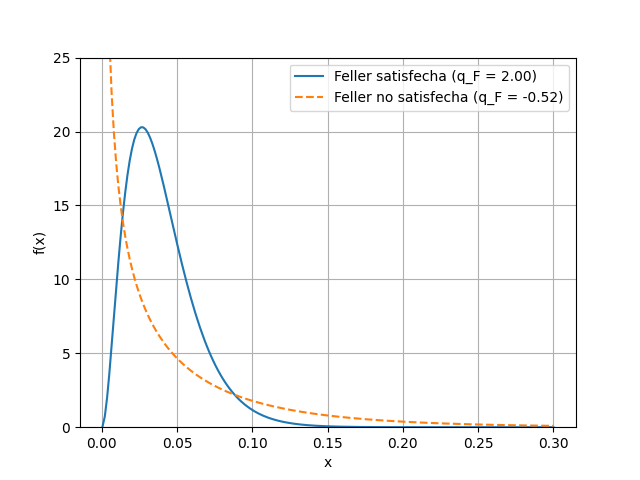
\includegraphics[width=0.8\textwidth]{cir_feller_density.png}
\caption{Función de densidad de probabilidad para $\gamma=0.2$ (condición satisfecha) y $\gamma=0.5$ (condición no satisfecha).}
\label{fig:cir_feller_density}
\end{figure}
Cuando se satisface la condición de Feller, la densidad queda concentrada en valores positivos y la probabilidad de que el proceso se acerque al origen es reducida. En cambio, cuando la condición no se cumple, la densidad presenta mayor masa cerca de cero, por lo que la varianza puede tomar valores muy pequeños. Este comportamiento es relevante en el modelo de Heston, y posteriormente en el modelo Heston--SLV, ya que el proceso CIR se utiliza para describir la varianza instantánea del subyacente.

\subsection{El modelo de Heston}

El modelo de Heston es uno de los modelos de volatilidad estocástica más utilizados en finanzas cuantitativas. Su principal idea consiste en sustituir la volatilidad constante del modelo de Black--Scholes por una varianza instantánea aleatoria que sigue un proceso CIR. Bajo la medida neutral al riesgo $\mathbb{Q}$, el modelo viene dado por el sistema de ecuaciones diferenciales estocásticas
\begin{equation}
\label{eq:heston_sv}
\begin{cases}
dS(t) = rS(t)\,dt+\sqrt{v(t)}S(t)\,dW^{S,\mathbb{Q}}(t), \\[0.15cm]
dv(t) = \kappa(\theta-v(t))\,dt+\gamma\sqrt{v(t)}\,dW^{v,\mathbb{Q}}(t),
\end{cases}
\end{equation}
con condiciones iniciales
\[
S(t_0)=S_0>0,
\qquad
v(t_0)=v_0>0.
\]

Los movimientos brownianos que aparecen en \ref{eq:heston_sv} están correlados según
\begin{equation}
\label{eq:heston_correlation}
dW^{S,\mathbb{Q}}(t)\,dW^{v,\mathbb{Q}}(t)=\rho_{S,v}\,dt.
\end{equation}

La primera ecuación describe la evolución del activo subyacente. Como estamos trabajando bajo la medida neutral al riesgo, la deriva del activo es el tipo libre de riesgo $r$. \medskip

La segunda ecuación describe la evolución de la varianza instantánea. Como se ha indicado, esta varianza sigue un proceso CIR, de modo que revierte hacia el nivel medio \(\theta\) con velocidad \(\kappa\) y presenta fluctuaciones aleatorias controladas por el parámetro \(\gamma\), conocido como volatilidad de la volatilidad. \medskip

\begin{observation}[Cambio de medida]
La formulación anterior se ha escrito directamente bajo la medida neutral al riesgo \(\mathbb{Q}\), ya que el objetivo del trabajo es la valoración de derivados y la calibración a precios de mercado. Esto es coherente con el marco introducido en el capítulo anterior: cuando se toma como numerario la cuenta bancaria libre de riesgo, la medida de valoración asociada es la medida neutral al riesgo, bajo la cual el precio descontado del activo debe ser una martingala.\medskip

En el modelo de Black--Scholes, el paso de la medida histórica \(\mathbb{P}\) a la medida neutral al riesgo \(\mathbb{Q}\) consiste, de forma esencial, en sustituir la deriva real \(\mu\) del activo por el tipo libre de riesgo \(r\):
\[
dS(t)=\mu S(t)\,dt+\sigma S(t)\,dW^{\mathbb{P}}(t),
\qquad
dS(t)=rS(t)\,dt+\sigma S(t)\,dW^{\mathbb{Q}}(t).
\]
En el modelo de Heston la idea es análoga, aunque más delicada, puesto que existen dos fuentes de aleatoriedad: una asociada al subyacente y otra asociada a la varianza.\medskip

Bajo la medida $\mathbb{P}$, la varianza podría escribirse con parámetros propios de la dinámica real del mercado. Sin embargo, al pasar a la medida de valoración, dichos parámetros pueden verse modificados por el cambio de medida. Por ello, en la práctica el modelo de Heston suele formularse directamente bajo \(\mathbb{Q}\), entendiendo que
\[
\kappa,\qquad \theta,\qquad \gamma,\qquad \rho_{S,v},\qquad v_0
\]
son parámetros de valoración calibrados a precios de opciones.
\end{observation}

\subsubsection{Ecuación de valoración de Heston}

Sea \(V(t,S,v)\) el valor de un derivado europeo escrito sobre el activo \(S\), suponiendo que la dinámica del par \((S(t),v(t))\) viene dada por el modelo de Heston. La ecuación de valoración asociada puede obtenerse mediante dos enfoques equivalentes: el enfoque de martingala y el enfoque de cobertura. Ambos procedimientos se desarrollan en \cite[pp.~245--247]{oosterlee2021modelos}; aquí se recoge únicamente la ecuación resultante, ya que la deducción sigue las mismas ideas introducidas para el modelo de Black--Scholes. \medskip

Desde el punto de vista de martingala, el valor descontado del derivado debe satisfacer
\begin{equation}
\label{eq:heston_expectation}
\frac{V(t,S(t),v(t))}{N(t)}
=
\mathbb{E}^{\mathbb{Q}}
\left[
\left.
\frac{V(T,S(T),v(T))}{N(T)}
\right|
\mathcal{F}_t
\right],
\end{equation}
donde \(N(t)\) representa la cuenta bancaria libre de riesgo. Si el tipo de interés \(r\) es constante, entonces \(N(t)=e^{rt}\), y la expresión anterior puede escribirse como
\[
V(t,S(t),v(t))
=
e^{-r(T-t)}
\mathbb{E}^{\mathbb{Q}}
\left[
V(T,S(T),v(T))
\mid
\mathcal{F}_t
\right].
\]

En particular, para un derivado europeo con payoff \(\Phi(S(T))\), se tiene la condición terminal
\[
V(T,S,v)=\Phi(S).
\]
Aplicando el lema de Itô bidimensional a \(V(t,S(t),v(t))\) y usando las dinámicas de \ref{eq:heston_sv}, se obtiene la siguiente ecuación en derivadas parciales:
\begin{equation}
\label{eq:heston_edp}
\frac{\partial V}{\partial t}
+rS\frac{\partial V}{\partial S}
+\kappa(\theta-v)\frac{\partial V}{\partial v}
+\frac{1}{2}vS^2\frac{\partial^2 V}{\partial S^2}
+\rho_{S,v}\gamma vS\frac{\partial^2 V}{\partial S\partial v}
+\frac{1}{2}\gamma^2v\frac{\partial^2 V}{\partial v^2}
-rV=0.
\end{equation}

El enfoque de cobertura conduce a la misma ecuación, aunque la construcción de la cartera replicante es más compleja que en Black--Scholes. En este caso existen dos fuentes de riesgo, una asociada al subyacente \(S(t)\) y otra asociada a la varianza \(v(t)\). Por tanto, si solo se negocian el activo subyacente y la cuenta bancaria, el mercado no permite cubrir directamente ambas fuentes de incertidumbre. Para completar la cobertura sería necesario incorporar algún instrumento adicional sensible a la volatilidad. Esta observación refleja la relación entre los modelos de volatilidad estocástica y la incompletitud de mercado. \medskip

La ecuación \ref{eq:heston_edp} también admite una interpretación probabilística mediante Feynman--Kac, que expresa el precio como una esperanza descontada bajo la medida neutral al riesgo. Además, una de las principales ventajas del modelo de Heston es que pertenece a la clase de modelos afines. Esto permite obtener su función característica en forma semianalítica, lo que facilita la valoración eficiente de opciones europeas y la posterior calibración del modelo a superficies de volatilidad implícita, por ejemplo mediante métodos basados en Fourier como el método COS.

\subsubsection*{Limitaciones del modelo de Heston}

El modelo de Heston introduce una fuente estocástica para la varianza y, por tanto, permite generar sonrisas y skews de volatilidad implícita que no pueden reproducirse en el modelo de Black--Scholes con volatilidad constante. Además, sus parámetros tienen una interpretación financiera clara: la correlación \(\rho_{S,v}\) influye principalmente en la inclinación del skew, la volatilidad de la volatilidad \(\gamma\) afecta a la curvatura de la sonrisa, \(v_0\) determina el nivel inicial de varianza, \(\theta\) representa el nivel de largo plazo y \(\kappa\) controla la velocidad de reversión hacia dicho nivel.

Sin embargo, aunque esta estructura proporciona una dinámica más rica que la de un modelo de volatilidad local puro, el modelo de Heston no garantiza por sí solo un ajuste exacto a toda la superficie de volatilidad implícita observada en mercado. En la práctica, la calibración se realiza escogiendo los parámetros
\[
\kappa,\qquad \theta,\qquad \gamma,\qquad \rho_{S,v},\qquad v_0
\]
de forma que los precios generados por el modelo se aproximen lo mejor posible a los precios de opciones cotizadas. No obstante, al tratarse de un modelo paramétrico con un número reducido de parámetros, puede no ser suficientemente flexible para reproducir con precisión todas las estructuras observadas en la superficie, especialmente cuando se consideran varios vencimientos y strikes.

Por tanto, el modelo de Heston presenta una ventaja importante frente a la volatilidad local: incorpora una dinámica estocástica de la varianza, lo que resulta especialmente relevante para productos sensibles a la evolución futura de la volatilidad. Sin embargo, también presenta una limitación: su capacidad de ajuste a la superficie inicial puede ser menor que la de un modelo de volatilidad local. Esta tensión entre ajuste inicial y dinámica futura motiva la introducción de los modelos de volatilidad local estocástica, que combinan una componente local, destinada a reproducir la superficie de mercado, con una componente estocástica, encargada de modelar la evolución aleatoria de la volatilidad.

%%%%%%%%%%%%%%%%%%%%%%%%%%%%%%%%%%%%%%%%%%%%%%%%%%%%%%%%%%%%%%%%%%%%%%%%%%%%%%%%%%%%%%%%

\section{Modelo de volatilidad local estocástica}

Los modelos de volatilidad local estocástica, conocidos como modelos \textit{Stochastic--Local Volatility} o SLV, combinan las ideas introducidas en las secciones anteriores. Por un lado, incorporan una componente local que permite ajustar la superficie de volatilidad implícita observada en mercado. Por otro lado, mantienen una componente estocástica para describir de forma más realista la evolución futura de la volatilidad.\medskip

Esta combinación permite corregir algunas de las limitaciones de los modelos LV y SV considerados por separado, y resulta especialmente útil en productos sensibles a la dinámica futura de la sonrisa de volatilidad, como las opciones \textit{forward-start}. En esta sección se introduce la formulación general del modelo SLV y, posteriormente, su particularización al caso Heston--SLV.

\subsection{Formulación general del modelo SLV}

Bajo la medida neutral al riesgo \(\mathbb{Q}\), un modelo de volatilidad local estocástica puede escribirse de forma general como
\begin{equation}
\label{eq:general_slv}
\begin{cases}
\dfrac{dS(t)}{S(t)}
=
r\,dt+\eta(S(t),t)\,\xi(v(t))\,dW^S(t), \\[0.25cm]
dv(t)
=
a_v(v(t),t)\,dt+b_v(v(t),t)\,dW^v(t), \\[0.25cm]
dW^S(t)\,dW^v(t)=\rho_{S,v}\,dt.
\end{cases}
\end{equation}

En esta formulación, \(S(t)\) representa el precio del activo subyacente y \(v(t)\) es el factor estocástico asociado a la volatilidad. La función \(\eta(S(t),t)\) representa la componente local del modelo, también denominada función de apalancamiento (leverage function).\medskip

Por otro lado, la función \(\xi(v(t))\) introduce la dependencia respecto del factor estocástico \(v(t)\), mientras que las funciones \(a_v\) y \(b_v\) determinan, respectivamente, la deriva y la difusión de dicho proceso. Finalmente, el parámetro \(\rho_{S,v}\in[-1,1]\) mide la correlación instantánea entre las dos fuentes de aleatoriedad.\medskip

El modelo \ref{eq:general_slv} contiene como casos particulares algunos de los modelos estudiados anteriormente. Si se toma \(\eta(S,t)=1\), se recupera un modelo puramente de volatilidad estocástica. En cambio, si la componente estocástica no introduce aleatoriedad adicional y se identifica el producto \(\eta(S,t)\xi(v(t))\) con la volatilidad local \(\sigma_{\mathrm{LV}}(S,t)\), se obtiene el modelo de volatilidad local.\medskip

Por tanto, el modelo SLV puede interpretarse como una extensión híbrida que combina la capacidad de ajuste de los modelos de volatilidad local con la dinámica de los modelos de volatilidad estocástica. En la siguiente subsección se estudia cómo se determina la componente local \(\eta\), que es el elemento que permite conectar ambas partes del modelo.

\subsection{Componente de volatilidad local del modelo}

El elemento que conecta la parte local y la parte estocástica del modelo SLV es la función \(\eta(S,t)\). Esta función se introduce para que el modelo reproduzca la superficie de volatilidad implícita observada en mercado, manteniendo al mismo tiempo una dinámica estocástica para la volatilidad.\medskip

La determinación de la función \(\eta\) se basa en la relación de consistencia entre el modelo SLV y el modelo de volatilidad local asociado a la superficie de mercado. Esta relación, conocida habitualmente como condición de proyección (Markovian projection), puede encontrarse en \cite[Sec.~10.2.1]{oosterlee2021modelos}. En particular, se impone que la varianza instantánea efectiva del modelo SLV, condicionada al nivel del subyacente, coincida con la varianza local obtenida mediante la fórmula de Dupire. Por tanto,
\begin{equation}
\label{eq:slv_projection}
\sigma_{\mathrm{LV}}^2(K,t)
=
\eta^2(K,t)\,
\mathbb{E}^{\mathbb{Q}}
\left[
\xi^2(v(t))\mid S(t)=K
\right].
\end{equation}

A partir de \ref{eq:slv_projection}, la componente local del modelo queda determinada por
\begin{equation}
\label{eq:eta_slv_general}
\eta(K,t)
=
\frac{
\sigma_{\mathrm{LV}}(K,t)
}{
\sqrt{
\mathbb{E}^{\mathbb{Q}}
\left[
\xi^2(v(t))\mid S(t)=K
\right]
}
}.
\end{equation}

En esta expresión, el numerador \(\sigma_{\mathrm{LV}}(K,t)\) es la función de volatilidad local introducida en la sección de volatilidad local. Por tanto, la componente local del modelo SLV hereda la información contenida en los precios de opciones vainilla observados inicialmente. \medskip

El papel de la función \(\eta\) no es sustituir a \(\sigma_{\mathrm{LV}}\), sino adaptar la componente estocástica del modelo para que, al condicionar por el nivel del subyacente, la varianza efectiva del modelo SLV coincida con la varianza local. De esta forma, la relación \ref{eq:slv_projection} permite combinar el ajuste inicial proporcionado por el modelo LV con la dinámica estocástica introducida por el proceso \(v(t)\).

El denominador, en cambio, depende de la componente estocástica del modelo. Concretamente, recoge el valor esperado de \(\xi^2(v(t))\) condicionado a que el subyacente tome el valor \(K\) en el instante \(t\). Este término no se conoce, en general, de forma explícita, ya que depende de la distribución conjunta de \((S(t),v(t))\) bajo el propio modelo SLV. Por ello, debe aproximarse numéricamente.

Una forma habitual de estimar esta esperanza condicional es mediante un procedimiento no paramétrico basado en simulaciones Monte Carlo. Para un instante temporal \(t_i\), se dispone de un conjunto de trayectorias simuladas
\[
\left(S_{j}(t_i),v_{j}(t_i)\right),
\qquad j=1,\ldots,N.
\]
Las trayectorias se agrupan según el valor alcanzado por el subyacente \(S_j(t_i)\), dividiendo el rango de valores simulados en intervalos o bins. Si \(I_k\) denota el \(k\)-ésimo bin y \(J_k=\{m:S_m(t_i)\in I_k\}\) es el conjunto de índices de las trayectorias que caen en dicho bin, entonces, para una trayectoria \(j\in J_k\), se aproxima
\begin{equation}
\label{eq:conditional_expectation_bins_general}
\mathbb{E}^{\mathbb{Q}}
\left[
\xi^2(v(t_i))\mid S(t_i)=S_{j}(t_i)
\right]
\approx
\frac{1}{N_k}
\sum_{m\in J_k}
\xi^2\left(v^{(m)}(t_i)\right),
\end{equation}
donde \(N_k\) es el número de trayectorias contenidas en dicho bin.

Así, para cada instante temporal y para cada nivel simulado del subyacente, la función \(\eta\) se calcula como el cociente entre la volatilidad local de mercado y la raíz cuadrada de la esperanza condicional estimada. En consecuencia, \(\eta\) actúa como un corrector local de la componente estocástica: ajusta el modelo para reproducir las volatilidades vainilla observadas, pero sin eliminar la aleatoriedad introducida por el proceso \(v(t)\).

\subsection{Modelo Heston--SLV}

En este trabajo se considera una particularización del modelo SLV en la que la componente estocástica de la volatilidad viene dada por el modelo de Heston. Es decir, se toma como factor estocástico la varianza instantánea \(v(t)\), cuya dinámica sigue un proceso CIR. En la formulación general \ref{eq:general_slv}, esto equivale a tomar
\[
\xi(v(t))=\sqrt{v(t)},
\qquad
a_v(v(t),t)=\kappa(\theta-v(t)),
\qquad
b_v(v(t),t)=\gamma\sqrt{v(t)}.
\]

Sustituyendo estas expresiones en el modelo SLV general, se obtiene el modelo Heston--SLV bajo la medida neutral al riesgo \(\mathbb{Q}\),
\begin{equation}
\label{eq:heston_slv}
\begin{cases}
\dfrac{dS(t)}{S(t)}
=
r\,dt+\eta(S(t),t)\sqrt{v(t)}\,dW^S(t), \\[0.25cm]
dv(t)
=
\kappa(\theta-v(t))\,dt+\gamma\sqrt{v(t)}\,dW^v(t), \\[0.25cm]
dW^S(t)\,dW^v(t)=\rho_{S,v}\,dt.
\end{cases}
\end{equation}

La primera ecuación describe la evolución del activo subyacente. La segunda ecuación coincide con la dinámica de la varianza en el modelo de Heston \ref{eq:heston_sv}. El parámetro \(\kappa\) representa la velocidad de reversión a la media, \(\theta\) el nivel medio de largo plazo, \(\gamma\) la volatilidad de la volatilidad y \(\rho_{S,v}\) la correlación instantánea entre el movimiento del subyacente y el de la varianza.

En este caso, como \(\xi^2(v(t))=v(t)\), la relación general para la componente local se simplifica a
\begin{equation}
\label{eq:heston_slv_leverage}
\eta(K,t)
=
\frac{
\sigma_{\mathrm{LV}}(K,t)
}{
\sqrt{
\mathbb{E}^{\mathbb{Q}}
\left[
v(t)\mid S(t)=K
\right]
}
}.
\end{equation}

Esta expresión muestra la estructura híbrida del modelo. El numerador \(\sigma_{\mathrm{LV}}(K,t)\) procede de la superficie de volatilidad local obtenida mediante Dupire y recoge la información de mercado contenida en las opciones vainilla. El denominador incorpora la información generada por la dinámica estocástica de Heston, a través de la esperanza condicional de la varianza dado el nivel del subyacente.

Por tanto, el modelo Heston--SLV puede interpretarse como una corrección local del modelo de Heston. La componente estocástica proporciona una dinámica más realista para la evolución futura de la volatilidad, mientras que la función \(\eta\) ajusta dicha dinámica para que sea consistente con la superficie de volatilidad implícita observada inicialmente. A continuación, describimos cómo se simula numéricamente este modelo mediante Monte Carlo.

\subsection{Simulación Monte Carlo del modelo}

La simulación del modelo Heston--SLV se realiza mediante un método de Monte Carlo. Para ello, se considera una partición uniforme del intervalo temporal \([0,T]\),
\[
0=t_0<t_1<\cdots<t_m=T,
\qquad
\Delta t=\frac{T}{m},
\]
y se simulan \(N\) trayectorias del par \((S(t),v(t))\). Denotaremos por
\[
S_{i,j}\approx S(t_j),
\qquad
v_{i,j}\approx v(t_j),
\]
el valor del subyacente y de la varianza en la trayectoria \(i\), con \(i=1,\ldots,N\), y en el instante \(t_j\), con \(j=0,\ldots,m\).

En cada instante temporal es necesario calcular la función de apalancamiento
\[
\eta(S_{i,j},t_j)
=
\frac{
\sigma_{\mathrm{LV}}(S_{i,j},t_j)
}{
\sqrt{
\mathbb{E}^{\mathbb{Q}}
\left[
v(t_j)\mid S(t_j)=S_{i,j}
\right]
}
}.
\]
El numerador \(\sigma_{\mathrm{LV}}(S_{i,j},t_j)\) procede de la superficie de volatilidad local obtenida mediante Dupire. El denominador, en cambio, depende de la distribución conjunta de \((S(t),v(t))\) bajo el modelo Heston--SLV y, en general, no se conoce de forma explícita.
%%%%%%%%%%%%
En cada instante \(t_j\), se aproxima la esperanza condicional mediante el estimador por bins descrito en \ref{eq:conditional_expectation_bins_general} y definimos
\[
\widehat{E}_{i,j}
=
\frac{1}{N_k^{(j)}}
\sum_{\ell\in J_k^{(j)}} v_{\ell,j}.
\]

Para introducir la correlación entre el movimiento del subyacente y el de la varianza, se generan dos variables normales estándar independientes,
\[
X_{i,j},Y_{i,j}\sim N(0,1).
\]
La fuente de aleatoriedad asociada al subyacente viene dada por \(X_{i,j}\), mientras que la correspondiente a la varianza se construye como
\[
\rho_{S,v}X_{i,j}
+
\sqrt{1-\rho_{S,v}^2}\,Y_{i,j}.
\]
De esta forma, ambas fuentes de aleatoriedad tienen correlación \(\rho_{S,v}\).

Aplicando un esquema de Euler a la dinámica Heston--SLV, se obtiene
\begin{equation}
\label{eq:euler_heston_slv_S}
S_{i,j+1}
=
S_{i,j}
+
rS_{i,j}\Delta t
+
\eta(S_{i,j},t_j)\sqrt{v_{i,j}}\,S_{i,j}\sqrt{\Delta t}\,X_{i,j},
\end{equation}
y
\begin{equation}
\label{eq:euler_heston_slv_v}
v_{i,j+1}
=
v_{i,j}
+
\kappa(\theta-v_{i,j})\Delta t
+
\gamma\sqrt{v_{i,j}}\sqrt{\Delta t}
\left(
\rho_{S,v}X_{i,j}
+
\sqrt{1-\rho_{S,v}^2}\,Y_{i,j}
\right).
\end{equation}

Sustituyendo la expresión discreta de \(\eta\), la ecuación del subyacente puede escribirse también como
\begin{equation}
\label{eq:euler_heston_slv_S_expanded}
S_{i,j+1}
=
S_{i,j}
+
rS_{i,j}\Delta t
+
\sqrt{
\frac{
\sigma_{\mathrm{LV}}^2(S_{i,j},t_j)
}{
\widehat{E}_{i,j}
}
}
S_{i,j}\sqrt{v_{i,j}}\sqrt{\Delta t}\,X_{i,j}.
\end{equation}
Esta forma muestra explícitamente cómo intervienen las dos componentes del modelo: la volatilidad local \(\sigma_{\mathrm{LV}}\), asociada a la superficie de mercado, y la esperanza condicional \(\widehat{E}_{i,j}\), asociada a la dinámica estocástica de la varianza.

Aunque el esquema anterior puede escribirse de forma aditiva para \(S_{i,j}\), también es habitual utilizar una versión exponencial del esquema. En ella, los coeficientes se evalúan al inicio de cada intervalo temporal y se mantienen constantes durante el paso \([t_j,t_{j+1}]\). Es decir, durante ese intervalo se toman como dados los valores
\[
\eta(S_{i,j},t_j),
\qquad
v_{i,j},
\qquad
r.
\]
Bajo esta aproximación, la actualización del subyacente viene dada por
\begin{equation}
\label{eq:log_euler_heston_slv}
S_{i,j+1}
=
S_{i,j}
\exp\left[
\left(
r-\frac{1}{2}\eta^2(S_{i,j},t_j)v_{i,j}
\right)\Delta t
+
\eta(S_{i,j},t_j)\sqrt{v_{i,j}}\sqrt{\Delta t}\,X_{i,j}
\right].
\end{equation}
Esta forma mantiene la positividad del subyacente y resulta natural para una dinámica de tipo lognormal con coeficientes constantes en cada paso temporal.\medskip

Además del esquema de Euler, se ha considerado también un esquema de tipo Almost Exact Simulation (AES), siguiendo el enfoque descrito en \cite[Sec.~10.2.3]{oosterlee2021modelos}. Este tipo de métodos busca reducir el sesgo de discretización asociado a la simulación del modelo Heston--SLV, especialmente en la componente de varianza y en la estimación de la esperanza condicional que aparece en la función de apalancamiento. Los detalles concretos de la implementación numérica y de los esquemas considerados se discutirán posteriormente.\medskip


Desde el punto de vista numérico, la simulación del proceso de varianza requiere cierto cuidado, ya que el proceso CIR debe permanecer no negativo. El tratamiento concreto utilizado para evitar valores negativos de la varianza se detallará posteriormente en la sección de implementación numérica.\medskip

Con esto queda definido el modelo Heston--SLV que se utilizará en el resto del trabajo. La construcción anterior muestra cómo se combinan la información de mercado recogida por la volatilidad local y la dinámica estocástica de la varianza propia del modelo de Heston. La valoración concreta de opciones vainilla y opciones de tipo \textit{forward-start} mediante las trayectorias simuladas se presentará más adelante, dentro del capítulo de implementación numérica, para poder compararla de forma directa con la valoración obtenida mediante Entropía Relativa Mínima.

\chapter{Entropía Relativa y Weighted Monte Carlo}

Como hemos visto en el capítulo de conceptos preliminares, y en particular en el Teorema~\ref{th:segundo-teorema-fundamental}, en mercados incompletos la medida martingala equivalente no tiene por qué ser única. En este contexto, la valoración de derivados no replicables puede interpretarse como un problema de selección de medida. La metodología de Entropía Relativa Mínima, conocida como Minimum Relative Entropy (MRE), proporciona un criterio para escoger una medida de valoración entre aquellas que son compatibles con la información de mercado disponible.\medskip

La idea del método es partir de una medida previa, asociada a un modelo inicial o prior, y construir una nueva medida que reproduzca determinadas restricciones de mercado, alejándose lo mínimo posible de la distribución original.\medskip

En la práctica, este enfoque puede implementarse mediante Weighted Monte Carlo (WMC). A diferencia de los modelos de Volatilidad Local Estocástica (SLV), donde la calibración modifica la dinámica del subyacente, WMC parte de un conjunto de trayectorias previamente simuladas y ajusta las probabilidades asignadas a cada una de ellas.\medskip

En este capítulo se presenta primero la formulación matemática del problema de Entropía Relativa Mínima descrita en \cite{articleAvellaneda}. A continuación, se describe su aplicación en el contexto Monte Carlo, se introducen las restricciones de calibración consideradas y se desarrolla la resolución numérica del problema dual.

\section{Formulación del problema de Entropía Relativa Mínima}

Antes de formular el problema de optimización asociado a la Entropía Relativa Mínima, introducimos primero el concepto de entropía de una variable aleatoria discreta.

\begin{definition}[Entropía de una variable aleatoria]
Sea \(X\) una variable aleatoria discreta definida sobre un espacio de probabilidad \((\Omega,\mathcal{F},\mathbb{P})\). Supongamos que \(\Omega\) es finito y que
\[
p(\omega)=\mathbb{P}(\{\omega\}), \qquad \omega\in\Omega.
\]
Se define la entropía de \(X\) como
\[
H(X)
:=
-\mathbb{E}^{\mathbb{P}}\left[\log p(\omega)\right]
=
-\sum_{\omega\in\Omega}
p(\omega)\log p(\omega).
\]
\end{definition}

Esta cantidad mide el grado de incertidumbre de la variable aleatoria. Si no hay incertidumbre, es decir, si toda la probabilidad está concentrada en un único estado, la entropía es nula. Por el contrario, la entropía alcanza su valor máximo cuando todos los estados tienen la misma probabilidad. En particular, si \(X\) es uniforme sobre un conjunto con \(n\) posibles estados, entonces
\[
H(X)=\log n.
\]

El concepto anterior puede extenderse para comparar dos medidas de probabilidad distintas. Esta extensión recibe el nombre de entropía relativa o divergencia de Kullback--Leibler.

\begin{definition}[Entropía relativa]
Sean \(\mathbb{P}\) y \(\mathbb{Q}\) dos medidas de probabilidad definidas sobre un mismo espacio finito \((\Omega,\mathcal{F})\). Denotamos por
\[
p(\omega)=\mathbb{P}(\{\omega\}),
\qquad
q(\omega)=\mathbb{Q}(\{\omega\})
\]
las probabilidades asociadas a cada estado \(\omega\in\Omega\). La entropía relativa de \(\mathbb{Q}\) respecto de \(\mathbb{P}\) se define como
\[
D(\mathbb{Q}\| \mathbb{P})
:=
\mathbb{E}^{\mathbb{Q}}
\left[
\log\left(\frac{q(\omega)}{p(\omega)}\right)
\right]
=
\sum_{\omega\in\Omega}
q(\omega)
\log\left(\frac{q(\omega)}{p(\omega)}\right).
\]
\end{definition}

La entropía relativa cuantifica la discrepancia entre una probabilidad previa \(\mathbb{P}\) y una probabilidad posterior \(\mathbb Q\). En este sentido, mide el coste de sustituir la probabilidad inicial por una nueva probabilidad. Además, verifica que es no negativa y
\[
D(\mathbb{Q}\| \mathbb{P}) = 0, \quad \text{si, y solo si, } \quad \mathbb{Q} = \mathbb P.
\]
La entropía relativa no es una distancia en sentido matemático, sino una divergencia estadística, ya que no es simétrica ni satisface, en general, la desigualdad triangular. Por tanto, minimizar la entropía relativa equivale a buscar una medida posterior lo más cercana posible a una medida previa, entendiendo dicha cercanía en el sentido de esta divergencia.\medskip


En el contexto de valoración de derivados, esta idea se utiliza para seleccionar una medida de probabilidad que reproduzca cierta información de mercado. Supongamos que partimos de una medida previa \(\mathbb{P}\), asociada a un modelo inicial, y queremos encontrar una nueva medida \(\mathbb{Q}\) bajo la cual se satisfagan determinadas restricciones de calibración.

Sea \(g_j(\omega)\) el valor descontado, o expresado en unidades del numerario, del \(j\)-ésimo instrumento de calibración en el escenario \(\omega\). Denotamos por \(c_j\) el precio objetivo de dicho instrumento, también expresado en unidades del numerario. Este precio puede ser una cotización de mercado o un precio de referencia generado por otro modelo. La condición de calibración se escribe entonces como
\[
\mathbb{E}^{\mathbb{Q}}\left[g_j(\omega)\right]=c_j,
\qquad j=1,\ldots,m.
\]
Es decir, la medida posterior debe valorar correctamente los instrumentos utilizados como restricciones.

Con esta notación, el problema de Entropía Relativa Mínima consiste en resolver
\[
\min_{\mathbb{Q}\in\mathcal{Q}}
D(\mathbb{Q}\|\mathbb{P})
\]
sujeto a
\[
\mathbb{E}^{\mathbb{Q}}\left[g_j(\omega)\right]=c_j,
\qquad j=1,\ldots,m.
\]
La familia \(\mathcal{Q}\) representa el conjunto de medidas de probabilidad admisibles. Por tanto, entre todas las medidas que reproducen las restricciones de mercado impuestas, se selecciona aquella que se mantiene más próxima a la medida previa \(\mathbb{P}\).

En particular, si una de las restricciones corresponde al activo subyacente y se toma como numerario la cuenta libre de riesgo, la condición anterior recupera la propiedad martingala del precio descontado. En el caso de tipo de interés constante \(r\), esta restricción puede escribirse como
\[
\mathbb{E}^{\mathbb{Q}}
\left[
e^{-rT}S(T)
\right]
=
S(0).
\]
De forma equivalente, si se trabaja directamente con precios descontados,
\[
\mathbb{E}^{\mathbb{Q}}
\left[
\frac{S(T)}{N(T)}
\right]
=
\frac{S(0)}{N(0)}.
\]
En el caso particular \(r=0\), y si no se consideran dividendos, esta condición se reduce a
\[
\mathbb{E}^{\mathbb{Q}}\left[S(T)\right]=S(0).
\]

Así, el problema MRE puede entenderse como un problema de selección de medida: se parte de una distribución previa y se busca una distribución posterior que respete las restricciones de mercado, como precios de opciones o condiciones forward, modificando lo mínimo posible la medida original.

\section{Weighted Monte Carlo}

Una vez formulado el problema de Entropía Relativa Mínima, pasamos a su implementación en el contexto de simulación Monte Carlo. La idea principal de Weighted Monte Carlo es partir de un conjunto de trayectorias simuladas bajo una medida previa y modificar únicamente las probabilidades asignadas a dichas trayectorias. De este modo, las trayectorias se mantienen fijas, pero la medida de probabilidad discreta cambia.

Supongamos que se generan \(N\) trayectorias del subyacente. En un Monte Carlo estándar, todas ellas reciben el mismo peso,
\[
p_i=\frac{1}{N}, \qquad i=1,\ldots,N.
\]
Sin embargo, en WMC se buscan nuevos pesos
\[
q=(q_1,\ldots,q_N),
\]
de forma que los instrumentos utilizados como benchmark sean valorados correctamente bajo la nueva medida.

Sean \(m\) los instrumentos de calibración y sea \(g_{ij}\) el payoff descontado del instrumento \(j\) en la trayectoria \(i\). La matriz de payoffs se define como
\begin{equation}
\label{matriz_payoffs_MRE}
  G=
\begin{pmatrix}
g_{11} & g_{12} & \cdots & g_{1m}\\
g_{21} & g_{22} & \cdots & g_{2m}\\
\vdots & \vdots & \ddots & \vdots\\
g_{N1} & g_{N2} & \cdots & g_{Nm}
\end{pmatrix}.  
\end{equation}


Denotamos \(C_j\) el precio objetivo del instrumento \(j\). De esta forma, las restricciones de calibración son
\[
\sum_{i=1}^N q_i g_{ij}=C_j,
\qquad j=1,\ldots,m.
\]

La matriz \(G\) no tiene por qué contener únicamente payoffs de opciones cotizadas, sino que también puede incluir restricciones auxiliares destinadas a asegurar propiedades financieras de la medida calibrada. Una de las más importantes es la condición de martingala, que garantiza la consistencia temporal del proceso bajo la medida posterior.

\begin{observation}
    Como se señala en \cite{articleElices}, al calibrar una medida posterior mediante Weighted Monte Carlo, el ajuste a opciones vainilla de distintos vencimientos no garantiza necesariamente que el proceso ponderado preserve la propiedad martingala. Por ello, pueden añadirse restricciones sintéticas adicionales cuyo precio objetivo es cero.

En particular, bajo una medida neutral al riesgo, el subyacente descontado debe ser martingala. Esta condición puede incorporarse a la matriz de calibración añadiendo columnas asociadas a payoffs sintéticos del tipo
\[
h_i^{k,\ell}
=
\mathbf{1}_{\{S_i(t_k)\in I_\ell\}}
\left(
S_i(t_{k+1})
\frac{F(0,t_k)}{F(0,t_{k+1})}
-
S_i(t_k)
\right),
\]
e imponiendo
\[
\sum_{i=1}^N q_i h_i^{k,\ell}=0.
\]
Estas restricciones no representan instrumentos cotizados, sino condiciones auxiliares para preservar de forma aproximada la propiedad martingala de la medida posterior.
\end{observation}

Con independencia del tipo concreto de restricciones incluidas en la matriz \(G\), el objetivo del método sigue siendo determinar los pesos \(q_i\) que modifican lo mínimo posible la medida previa y que satisfacen las condiciones de calibración impuestas. En el caso de una medida previa general \(p=(p_1,\ldots,p_N)\), el problema se escribe como

\begin{equation}
\label{eq:problema_minimizacion_wmc}
   \min_q D(q\|p) = \min_{q}
    \sum_{i=1}^N q_i
    \log\left(\frac{q_i}{p_i}\right)
\end{equation}

sujeto a
\[
\sum_{i=1}^N q_i=1,\quad q_i\geq 0,\,
\qquad i=1,\ldots,N;
\]
\[
\sum_{i=1}^N q_i g_{ij}=C_j,
\qquad j=1,\ldots,m,
\]

En el caso básico de WMC, la medida previa es uniforme, es decir, \(\displaystyle p_i=\frac{1}{N}\). Por tanto, el término constante \(\log N\) puede omitirse y el problema equivale a 
\[
 \min_q\sum_{i=1}^N q_i\log q_i
\]
bajo las mismas restricciones de calibración.

\subsection*{Resolución mediante multiplicadores de Lagrange}

El problema de Entropía Relativa Mínima planteado anteriormente es un problema de optimización convexa con restricciones lineales. Siguiendo la formulación de \cite{articleAvellaneda}, puede resolverse mediante su problema dual, introduciendo multiplicadores de Lagrange asociados a las restricciones de calibración.\medskip

Introducimos un vector de multiplicadores de Lagrange
\[
\lambda=(\lambda_1,\ldots,\lambda_m),
\]
asociado a estas restricciones. Para un valor dado de \(\lambda\), el vector de probabilidades posterior que resuelve el problema tiene forma exponencial, también conocida como forma de Boltzmann--Gibbs:
\begin{equation*}
\displaystyle
    q_i
=
\frac{
p_i\exp\left(\sum_{j=1}^m \lambda_j g_{ij}\right)
}{
Z(\lambda)
},
\qquad i=1,\ldots,N,
\end{equation*}
donde \(Z(\lambda)\) es el factor de normalización dado por
\[
Z(\lambda)
=
\sum_{i=1}^N
p_i
\exp\left(\sum_{j=1}^m \lambda_j g_{ij}\right).
\]
En el caso particular de un prior uniforme, \(\displaystyle p_i=\frac{1}{N}\), se obtiene
\[
Z(\lambda)
=
\frac{1}{N}
\sum_{i=1}^N
\exp\left(\sum_{j=1}^m \lambda_j g_{ij}\right),
\]
y
\[
q_i
=
\frac{
\exp\left(\sum_{j=1}^m \lambda_j g_{ij}\right)
}{
\sum_{\ell=1}^N
\exp\left(\sum_{j=1}^m \lambda_j g_{\ell j}\right)
}.
\]

Por tanto, el problema original puede reformularse como un problema sin restricciones en los multiplicadores de Lagrange. Definimos la función dual
\[
W(\lambda)
:=
\log Z(\lambda)
-
\sum_{j=1}^m \lambda_j C_j.
\]
El objetivo es entonces resolver
\[
\min_{\lambda\in\mathbb{R}^m} W(\lambda).
\]
Denotaremos por \(\lambda^*\) al valor de los multiplicadores de Lagrange que minimiza la función \(W\).

En \cite{articleAvellaneda} se muestra que esta formulación permite recuperar las restricciones de calibración impuestas previamente. En particular, cuando los precios objetivo son consistentes, el mínimo existe y es único.

\subsection{Formulaciones de calibración: ajuste exacto y ajuste ponderado}

La formulación anterior corresponde al caso de ajuste exacto, conocido en \cite{articleAvellaneda} como \textit{exact fitting}. En este caso se exige que todos los instrumentos benchmark sean reproducidos exactamente bajo la medida posterior. En forma matricial, esta condición se escribe como
\[
G^\top q=C,
\]
donde \(G=(g_{ij})\), \(q=(q_1,\ldots,q_N)^\top\) y \(C=(C_1,\ldots,C_m)^\top\). Por tanto, en el ajuste exacto la calibración se obtiene resolviendo
\[
\min_{\lambda} W(\lambda),
\]
y el mínimo debe verificar
\[
\nabla W(\lambda)=G^\top q-C=0.
\]

Sin embargo, en la práctica puede ser conveniente relajar las restricciones de calibración. Esto ocurre, por ejemplo, cuando el número de restricciones es elevado, cuando algunas de ellas son casi redundantes o cuando se desea permitir cierta tolerancia numérica en los precios objetivo. Para ello se considera una segunda formulación, denominada \textit{weighted least squares}, en la que las desviaciones respecto a los precios benchmark se controlan mediante parámetros de tolerancia. \medskip

En esta versión, la función objetivo dual se modifica añadiendo un término cuadrático en los multiplicadores:
\[
H(\lambda)
=
W(\lambda)
+
\frac{1}{2}
\sum_{j=1}^m
\omega_j\lambda_j^2,
\]
donde \(\omega_j>0\) representa el parámetro de regularización asociado a la restricción \(j\). En forma matricial,
\[
H(\lambda)
=
W(\lambda)
+
\frac{1}{2}\lambda^\top\Omega\lambda,
\]
con
\[
\Omega=\operatorname{diag}(\omega_1,\ldots,\omega_m).
\]
El gradiente de esta nueva función objetivo es
\[
\nabla H(\lambda)
=
G^\top q-C+\Omega\lambda.
\]
Por tanto, en el óptimo ya no se impone necesariamente \(G^\top q=C\), sino que se cumple
\[
G^\top q-C
=
-\Omega\lambda.
\]
Así, el error de calibración queda controlado por los parámetros \(\omega_j\). Con esta convención, \(\Omega=0\) recupera el ajuste exacto, mientras que valores positivos introducen una regularización del problema dual.

La Hessiana correspondiente viene dada por
\[
\nabla^2H(\lambda)
=
\nabla^2W(\lambda)+\Omega.
\]
Por tanto, el ajuste ponderado puede interpretarse como una versión regularizada del ajuste exacto.

%%%%%%%%%%%%%%%%%%%%%%%%%%%%%%%%%%%%%%%%%%%%%%%%%%%%%%%%%%%%%%%%%%%%%%%%%%

\subsection{Resolución numérica del problema dual}

Una vez elegida la formulación de calibración, el problema se resuelve numéricamente en términos de los multiplicadores de Lagrange. Para ello se utiliza un método iterativo de tipo Newton, basado en el gradiente y la Hessiana de la función objetivo.

La idea consiste en aproximar la función dual mediante su desarrollo de Taylor de segundo orden alrededor de un punto \(\widehat{\lambda}\). En el caso del ajuste exacto, la condición de primer orden asociada a esta aproximación cuadrática conduce a
\[
0
=
\nabla W(\widehat{\lambda})
+
J(\widehat{\lambda})(\lambda-\widehat{\lambda}),
\]
donde
\[
J(\widehat{\lambda})=\nabla^2 W(\widehat{\lambda}).
\]
De esta expresión se obtiene el paso de Newton
\[
\lambda
=
\widehat{\lambda}
-
J(\widehat{\lambda})^{-1}\nabla W(\widehat{\lambda}).
\]

En forma iterativa, tomando \(\widehat{\lambda}=\lambda^{(k)}\), el paso de Newton se calcula resolviendo
\[
J(\lambda^{(k)})d^{(k)}
=
\nabla W(\lambda^{(k)}),
\]
donde
\[
J(\lambda^{(k)})=\nabla^2 W(\lambda^{(k)}).
\]
Después se actualizan los multiplicadores mediante
\[
\lambda^{(k+1)}
=
\lambda^{(k)}
-
\alpha d^{(k)},
\]
donde \(\alpha\in(0,1]\) es un parámetro de relajación.\medskip

En el caso de mínimos cuadrados ponderados, se procede de forma análoga, sustituyendo \(W\) por \(H\). Por tanto, se resuelve
\[
J_H(\lambda^{(k)})d^{(k)}
=
\nabla H(\lambda^{(k)}),
\]
con
\[
J_H(\lambda^{(k)})
=
\nabla^2 H(\lambda^{(k)}),
\]
y se actualiza
\[
\lambda^{(k+1)}
=
\lambda^{(k)}
-
\alpha d^{(k)}.
\]

En la implementación, el parámetro \(\alpha\) se utiliza para amortiguar el paso de Newton y mejorar la estabilidad del procedimiento. Además, el cálculo de \(\log Z(\lambda)\) se evalúa de forma estable para evitar problemas numéricos al calcular exponenciales. También se incorporan salvaguardas numéricas, como una pequeña regularización diagonal del sistema lineal y, en caso necesario, la resolución mediante mínimos cuadrados cuando el sistema está mal condicionado.\medskip

El algoritmo se detiene cuando el gradiente es suficientemente pequeño o cuando el error de calibración queda por debajo de la tolerancia fijada. Una vez alcanzada la convergencia, se obtiene el vector óptimo de multiplicadores \(\lambda^*\) y, sustituyéndolo en la expresión exponencial de los pesos, se calculan las probabilidades posteriores finales \(q_i\).

%%%%%%%%%%%%%%%%%%%%%%%%%%%%%%%%%%%%%%%%%%%%%%%%%%%%%%%%%%%%%%%%%%%%%%%%%%%%%%%

\subsection{Esquema del algoritmo}

El procedimiento de calibración puede resumirse en los siguientes pasos:

\begin{enumerate}
    \item Simular \(N\) trayectorias del subyacente bajo la medida previa.

    \item Calcular los payoffs descontados de los instrumentos benchmark en cada trayectoria y construir la matriz
    \[
    G=(g_{ij}).
    \]

    \item Fijar los precios objetivo de los instrumentos de calibración,
    \[
    C=(C_1,\ldots,C_m).
    \]

    \item Inicializar los multiplicadores de Lagrange, normalmente con
    \[
    \lambda^{(0)}=0.
    \]

    \item En cada iteración, calcular los pesos \(q_i\), el gradiente y la Hessiana de la función objetivo correspondiente, \(W\) en el caso de ajuste exacto o \(H\) en el caso ponderado.

    \item Actualizar los multiplicadores mediante un paso de Newton amortiguado.

    \item Repetir el proceso hasta que el gradiente o el error de calibración sean suficientemente pequeños.

    \item Una vez alcanzada la convergencia, obtener los pesos posteriores calibrados \(q_i\).
\end{enumerate}

La formulación dual, el ajuste exacto y la versión de mínimos cuadrados ponderados siguen la metodología de Weighted Monte Carlo descrita en \cite{articleAvellaneda}. Asimismo, el uso de un esquema iterativo basado en el gradiente y la Hessiana se encuentra en línea con las implementaciones descritas en \cite{articleElices}. En este trabajo se incorporan además algunas salvaguardas numéricas propias de la implementación, como la evaluación estable de la función de normalización, la amortiguación del paso de Newton y una regularización diagonal en los sistemas lineales cuando resulta necesario.\medskip

Con esto queda definida la metodología de Entropía Relativa Mínima. La valoración concreta de opciones vainilla y opciones de tipo \textit{forward-start} bajo la medida posterior está desarrollada en el capítulo de implementación numérica.

\chapter{Implementación numérica y resultados}

En este capítulo se presentan los resultados numéricos obtenidos al aplicar las dos metodologías estudiadas en los capítulos anteriores: el modelo de Volatilidad Local Estocástica y el enfoque de Entropía Relativa Mínima implementado mediante Weighted Monte Carlo. El objetivo es mostrar cómo se han utilizado los datos de mercado disponibles, cómo se han calibrado ambos métodos y cómo se comparan los precios resultantes para distintos instrumentos derivados.\medskip

Antes de presentar los resultados numéricos, se introduce la medida de error utilizada para evaluar la calidad de ajuste de los modelos y para comparar los precios obtenidos por las distintas metodologías. 

\section{Medidas de error} 

Para cuantificar la diferencia entre los precios obtenidos mediante los distintos métodos se utilizará el error absoluto. Dado un instrumento financiero $k$, denotaremos por $V_k^{\mathrm{mkt}}$ su precio de mercado y por $V_k^{\mathrm{mod}}$ el precio obtenido mediante el modelo o metodología considerada. El error absoluto asociado a dicho instrumento se define como 
\begin{equation} 
e_k = \left| V_k^{\mathrm{mkt}} - V_k^{\mathrm{mod}} \right|. \label{eq:error_absoluto} 
\end{equation}
Esta cantidad mide la discrepancia, en valor absoluto, entre ambos precios. Esta será la noción de error que se mostrará en las tablas de resultados, tanto en el capítulo como en los apéndices. 

Cuando se comparen varios instrumentos de forma conjunta, se empleará el error absoluto medio, conocido como Mean Absolute Error (MAE). Si se consideran $n$ instrumentos, el MAE se define como 
\begin{equation} 
\mathrm{MAE} = \frac{1}{n} \sum_{k=1}^{n} \left| V_k^{\mathrm{mod}} - V_k^{\mathrm{ref}} \right|. \label{eq:mae} \end{equation}
Se utilizará para comparar de forma global los precios obtenidos mediante el modelo Heston--SLV y mediante el método de Entropía Relativa Mínima, así como para evaluar la proximidad de cada metodología respecto a los precios de mercado considerados.

\section{Implementación del modelo Heston--SLV}

En esta sección describimos la implementación numérica del modelo Heston--SLV introducido previamente. Como se explicó en el capítulo anterior, este modelo combina una componente de volatilidad estocástica de tipo Heston con una corrección local que permite incorporar la información contenida en la superficie de volatilidad implícita.

La implementación seguida consta de tres pasos principales. En primer lugar, construimos los precios de referencia a partir de una matriz de volatilidades implícitas. En segundo lugar, calibramos los parámetros de la componente Heston y calculamos la varianza local asociada a la superficie de precios. Finalmente, podemos simular trayectorias bajo la dinámica Heston--SLV y valorar los instrumentos considerados mediante Monte Carlo.

\subsection{Datos de entrada y precios de referencia}

Como datos de entrada se toma la matriz de volatilidades implícitas considerada en \cite[Cap. 8, Tabla 8.1]{oosterlee2021modelos}, asociada a distintos vencimientos y precios de ejercicio. En la implementación se fija $S_0=100$ y $r=0$, y las volatilidades, expresadas inicialmente en porcentaje, se transforman a escala decimal para realizar los cálculos.

Las volatilidades consideradas son las siguientes:

\begin{table}[H]
\centering
\small
\begin{tabular}{c|cccccccc}
\hline
\textbf{Strike / T} & \textbf{1w} & \textbf{1m} & \textbf{6m} & \textbf{1y} & \textbf{2y} & \textbf{5y} & \textbf{8y} & \textbf{10y} \\
\hline
40  & 22.622 & 22.371 & 20.706 & 18.537 & 18.041 & 16.395 & 14.491 & 13.136 \\
60  & 15.491 & 15.350 & 14.415 & 13.195 & 12.916 & 11.988 & 10.917 & 10.177 \\
80  & 9.930  & 9.882  & 9.562  & 9.154  & 9.070  & 8.786  & 8.459  & 8.251  \\
100 & 5.001  & 5.070  & 5.515  & 6.041  & 6.196  & 6.639  & 7.015  & 7.221  \\
120 & 4.542  & 4.598  & 4.962  & 5.430  & 5.654  & 6.277  & 6.782  & 7.041  \\
140 & 6.278  & 6.300  & 6.405  & 6.460  & 6.607  & 6.982  & 7.232  & 7.328  \\
160 & 7.748  & 7.752  & 7.707  & 7.517  & 7.615  & 7.806  & 7.824  & 7.751  \\
180 & 8.988  & 8.976  & 8.818  & 8.445  & 8.508  & 8.563  & 8.399  & 8.182  \\
\hline
\end{tabular}
\caption{Superficie de volatilidades implícitas de mercado, expresadas en porcentaje.}
\label{tab:volatilidades_implicitas_mercado}
\end{table}

A partir de esta superficie de volatilidades se construye una superficie de precios de opciones call mediante la fórmula de Black--Scholes presentada en Teorema \ref{th:ecuacion-black-scholes}. En concreto, para cada vencimiento $T_i$ y cada strike $K_j$, se obtiene un precio
\[
    C_{ij}^{\mathrm{mkt}}
    =
    C^{\mathrm{BS}}
    \left(
        S_0,K_j,T_i,r,\sigma_{\mathrm{imp}}(T_i,K_j)
    \right).
\]

Estos precios se consideran como precios de mercado o precios de referencia en la implementación del modelo Heston--SLV. De esta forma, la calibración y la posterior comparación se realizan frente a una superficie de precios coherente con la matriz de volatilidades implícitas inicial.

\subsection{Calibración de la componente Heston}

Una vez construida la superficie de precios de referencia, se calibra la componente de volatilidad estocástica del modelo. Para ello se considera el modelo de Heston--SLV \ref{eq:heston_slv}.

La calibración consiste en buscar los parámetros
\[
    \kappa,\quad \theta,\quad \gamma,\quad \rho_{S,v},\quad v_0,
\]
que minimizan la diferencia entre los precios de referencia $C_{ij}^{\mathrm{mkt}}$ y los precios generados por el modelo de Heston. Para calcular estos últimos empleamos el método COS, utilizando la función característica del modelo.

El problema de calibración se plantea de forma esquemática como
\begin{equation}
    \min_{\kappa,\theta,\gamma,\rho_{S,v},v_0}
    \left(
    \sum_{i,j}
    \left(
        C_{ij}^{\mathrm{Heston}}
        -
        C_{ij}^{\mathrm{mkt}}
    \right)^2
    \right)^{1/2}.
    \label{eq:calibracion_heston_slv_impl}
\end{equation}

En la implementación se impone además la condición de Feller \ref{eq:feller_condition} con el objetivo de favorecer la positividad del proceso de varianza.

Los parámetros obtenidos en la calibración son los que se muestran en la Tabla \ref{tab:parametros_heston_slv}.

\begin{table}[H]
\centering
\begin{tabular}{c c c c c c}
\hline
$\kappa$ & $\theta$ & $\gamma$ & $\rho_{S,v}$ & $v_0$ \\
\hline
$2.12$ & $0.06$ & $0.16$ & $-0.71$ & $0.001$ \\
\hline
\end{tabular}
\caption{Parámetros calibrados de la componente Heston.}
\label{tab:parametros_heston_slv}
\end{table}
%%%%%%%%%%%%%%%%%%%%%%%%55

\subsection{Construcción numérica de la función de apalancamiento}

En la implementación, la función de apalancamiento se construye directamente a partir de la expresión obtenida anteriormente en \ref{eq:eta_slv_general}.

En primer lugar, la superficie de volatilidad implícita de mercado se transforma en una superficie de precios call mediante la fórmula de Black--Scholes. A partir de esta superficie de precios se aplica la fórmula de Dupire para obtener la varianza local \(\sigma_{\mathrm{LV}}^2(T,K)\). Sin embargo, en las primeras pruebas numéricas se observó que aplicar Dupire directamente sobre la malla original de strikes producía valores inestables cerca de precios ATM.

Por lo tanto, introducimos una malla intermedia más fina en la dirección de los strikes. En concreto, para cada vencimiento se interpola la superficie de volatilidad implícita por interpolación cúbica tipo Hermite y se evalúa en una malla con paso \(\Delta K=2.5\). Después se reconstruyen los precios Black--Scholes sobre esa malla refinada y se aplica Dupire sobre la nueva superficie. 

Esta elección se apoya en \cite{SaporitoYangZubelli2017,Corlay2013}, donde se estudia la calibración de modelos SLV y subraya la importancia de interpolar y estabilizar la superficie antes de construir la función de apalancamiento; y en el interpolante cúbico descrito en \cite{FritschButland1984}.\medskip

De esta forma, la varianza local obtenida cerca de ATM resulta mucho más estable. Por ejemplo, para \(K=100\), los valores obtenidos son:
\[
\begin{array}{c|cccccc}
\text{Vencimiento} & 6m & 1y & 2y & 5y & 8y & 10y \\
\hline
\sigma_{\mathrm{LV}}^2(T,100)
& 0.0045 & 0.0046 & 0.0042 & 0.0047 & 0.0052 & 0.0055
\end{array}
\]

Una vez calculada la superficie local, el denominador de la función de apalancamiento se estima durante la simulación Monte Carlo. En cada fecha de la malla temporal se dispone de los valores simulados
\[
(S_{i,j},V_{i,j}), \qquad i=1,\ldots,N.
\]
Las trayectorias se ordenan según el valor del subyacente \(S_{i,j}\) y se dividen en un número fijo de grupos o bins. Dentro de cada grupo se calcula la media de las varianzas simuladas. Así, si \(B_k^{(j)}\) es el conjunto de trayectorias que caen en el \(k\)-ésimo bin en el instante \(t_j\), para una trayectoria \(i\in B_k^{(j)}\) se aproxima
\[
\widehat E_{i,j}
=
\frac{1}{|B_k^{(j)}|}
\sum_{m\in B_k^{(j)}} V_{m,j}.
\]
Esta cantidad aproxima
\[
\mathbb{E}^{\mathbb{Q}}[V_{t_j}\mid S_{t_j}=S_{i,j}].
\]

Finalmente, para cada trayectoria y cada instante temporal, la función de apalancamiento utilizada en la simulación se calcula como
\[
\eta_{i,j}
=
\frac{\sigma_{\mathrm{LV}}(t_j,S_{i,j})}
{\sqrt{\max\{\widehat E_{i,j},\epsilon\}}},
\]
donde \(\epsilon\) es una constante pequeña introducida para evitar divisiones por valores próximos a cero. Por tanto, el resultado de esta etapa no es un único valor de \(\eta\), sino una matriz de valores \(\eta_{i,j}\), uno para cada trayectoria y cada instante de simulación. Esta matriz se actualiza dinámicamente a medida que evolucionan las trayectorias del modelo Heston--SLV.


%%%%%%%%%%%%%%%%%%%%%%%%%%%%%%%%%%%%%%%%%%%%%%%%%%%%%%%

\subsection{Simulación Monte Carlo del modelo Heston--SLV}

Una vez calibrada la componente Heston y construida la función de apalancamiento, se simulan trayectorias bajo el modelo Heston--SLV definido en \ref{eq:heston_slv}. Para ello se considera una malla temporal que contiene los vencimientos empleados en la valoración y se simulan conjuntamente las trayectorias del subyacente y de la varianza.

En cada paso temporal se evalúa la función de apalancamiento a partir de la volatilidad local y de la estimación de la esperanza condicional de la varianza. De esta forma, la difusión del subyacente incorpora simultáneamente la componente estocástica de Heston y la corrección local necesaria para reproducir la superficie de mercado.

En la implementación se han considerado dos esquemas de simulación. El primero es un esquema de Euler, que proporciona una discretización directa de la dinámica y evita problemas numéricos asociados a valores negativos de la varianza. El segundo es un esquema Almost Exact Simulation (AES), en el que la componente CIR de la varianza se simula de forma más precisa.

Para comparar ambos métodos hemos analizado las volatilidades implícitas que se obtienen de dichos precios. 

\begin{figure}[H]
    \centering
    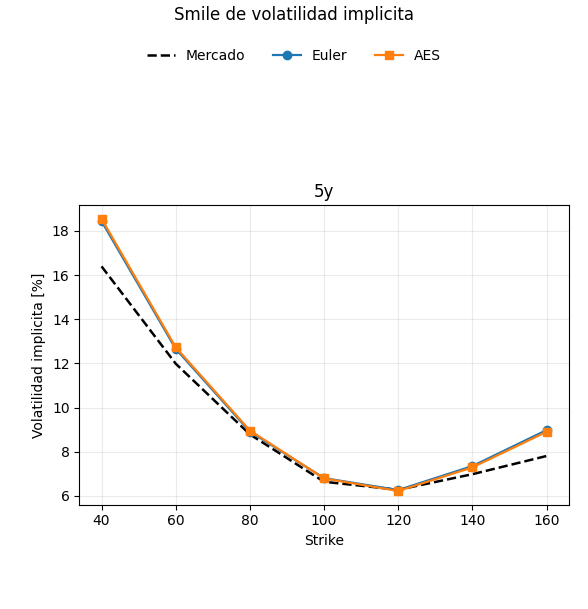
\includegraphics[width=0.5\textwidth]{AES_vs_Euler_5y.png}
    \caption{Comparación del smile de volatilidad implícita obtenido con los esquemas Euler y AES frente al smile de mercado para un vencimiento $T = 5$.}
    \label{fig:aes_euler_smile}
\end{figure}

Como se observa en la Figura \ref{fig:aes_euler_smile}, las curvas obtenidas con Euler y AES son prácticamente coincidentes para los strikes considerados. Además, ambas reproducen de forma adecuada la estructura decreciente y posterior recuperación del smile de mercado. Las pequeñas diferencias entre los dos esquemas son reducidas en comparación con el nivel de volatilidad implícita y pueden atribuirse al error de discretización y al error Monte Carlo de la simulación.\medskip

Por tanto, en este caso la elección entre Euler y AES no modifica de forma significativa los resultados finales en términos de volatilidad implícita. A continuación, se muestran y se estudian los resultados obtenidos por el esquema de Euler. \medskip

Además, tras cada paso temporal reescalamos las trayectorias de \(S(t)\) para que su media coincida con el valor
\[
    \mathbb{E}^{\mathbb{Q}}[S(t)] = S_0 e^{rt}.
\]

\subsection{Resultados obtenidos}

Los resultados principales de esta implementación son los parámetros calibrados de la componente Heston, la matriz de varianzas locales obtenida mediante Dupire y los precios de las opciones valoradas bajo el modelo Heston--SLV.

Para cada opción considerada se calcula el error absoluto entre el precio de referencia y el precio obtenido mediante SLV, siguiendo la definición dada en \ref{eq:error_absoluto}. Asimismo, para resumir el ajuste global del modelo se calcula el error absoluto medio, conforme a \ref{eq:mae}.

Las tablas completas con los precios de mercado, los precios obtenidos mediante Heston--SLV y los errores correspondientes se incluyen en las Tablas \ref{tab:slv_ref_put} y \ref{tab:slv_vs_bs_call}. 
%%%%%%%%%%%%%%%%%%%%%%%%%%%%%%%%%%%%%%%%%%%%%%%%%%%%%%
\section{Implementación del método MRE}
\label{sec:implementacion_mre}

Una vez presentada anteriormente la formulación del método de Entropía Relativa Mínima y su implementación mediante Weighted Monte Carlo en esta sección describimos cómo se ha llevado a cabo su implementación numérica. \medskip

La idea central de la implementación es mantener fijas las trayectorias simuladas del subyacente y modificar únicamente las probabilidades asociadas a cada una de ellas. Por tanto, frente al modelo Heston--SLV, donde la calibración afecta directamente a la dinámica simulada, el método MRE actúa sobre la medida discreta definida por las trayectorias Monte Carlo.

\subsection{Datos de entrada y configuración inicial}

Para que la comparación con el modelo Heston--SLV sea homogénea, se utiliza el mismo valor inicial del subyacente,
\[
S_0=100,
\]
y se consideran tipo de interés libre de riesgo y tasa de dividendos nulos,
\[
r=0, \qquad q=0.
\]
La calibración se realiza con opciones europeas de tipo call. Los vencimientos considerados son
\[
T\in
\left\{
\frac{1}{52},
\frac{1}{12},
0.5,
1,
2,
5,
8,
10
\right\},
\]
que corresponden a \(1w\), \(1m\), \(6m\), \(1y\), \(2y\), \(5y\), \(8y\) y \(10y\). Los strikes utilizados como benchmark son
\[
K\in\{40,60,80,100,120,140\}.
\]

Los precios objetivo empleados en la calibración MRE son los precios obtenidos previamente con la simulación Heston--SLV para esos mismos strikes y vencimientos. De este modo, la medida posterior MRE se calibra frente a la misma referencia que después se utilizará en la comparación entre metodologías.

La simulación previa se realiza con un modelo lognormal bajo medida neutral al riesgo. En la implementación se utilizan \(N=20000\) trayectorias, una semilla fija igual a \(12345\) y variables antitéticas, con el objetivo de mejorar la reproducibilidad y reducir la variabilidad Monte Carlo. Además, en lugar de utilizar una volatilidad prior constante para todos los vencimientos, se construye una estructura temporal de volatilidad ATM a partir de los propios precios benchmark. Como valor auxiliar de respaldo se fija
\[
\sigma_{\mathrm{prior}}=0.50,
\]
que solo se utiliza si no puede extraerse alguna volatilidad implícita representativa.

\subsection{Construcción de la medida previa}

La medida previa se define sobre las trayectorias simuladas. Inicialmente, y antes de incorporar la información de mercado, todas las trayectorias se consideran equiprobables, de modo que
\[
p_i=\frac{1}{N}, \qquad i=1,\ldots,N.
\]
A continuación, sobre cada una de estas trayectorias evaluamos los payoffs descontados de las opciones benchmark consideradas en la calibración. De esta forma, construimos la matriz \(G\), denominada matriz de payoffs, cuya estructura se recoge en \ref{matriz_payoffs_MRE}.\medskip
%miarar bien lo de arbitraje

Antes de construir la matriz de payoffs utilizada en la calibración MRE, se incorpora un módulo de comprobación de arbitraje estático sobre el conjunto finito de precios benchmark. El objetivo de este paso es verificar que los precios de mercado empleados como restricciones son compatibles con, al menos, una medida de valoración libre de arbitraje. Esta comprobación se realiza antes de la interpolación o calibración, ya que un conjunto de precios con arbitraje puede impedir la convergencia del problema de entropía relativa o generar pesos posteriores financieramente inconsistentes.

Para ello, trabajamos con precios normalizados por vencimiento. Si $(D_j)$ es el factor de descuento y $(F_j)$ el forward asociado al vencimiento $(T_j)$, se define
\[
k=\frac{K}{F_j},
\qquad
c_j(k)=\frac{C_j(K)}{D_jF_j}.
\]

Las condiciones de arbitraje estático comprobadas son las siguientes:

\begin{itemize}
\item Ausencia de arbitraje vertical: para cada vencimiento, los precios de las calls normalizadas deben ser decrecientes respecto al strike. Si se ordenan los strikes normalizados como
\[
0=k_0<k_1<\cdots<k_n,
\qquad c_0=1,
\]
y se definen las pendientes discretas
\[
q_i=\frac{c_{i-1}-c_i}{k_i-k_{i-1}},
\qquad i=1,\ldots,n,
\]
debe cumplirse
\[
0\leq q_i\leq 1.
\]

\item Ausencia de arbitraje butterfly: para cada vencimiento, la función de precios normalizados debe ser convexa respecto al strike. En términos de las pendientes anteriores, esta condición equivale a exigir
\[
1\geq q_1\geq q_2\geq \cdots \geq q_n\geq 0.
\]

\item Ausencia de arbitraje calendario: para vencimientos consecutivos \(T_j<T_{j+1}\), y sobre una misma malla de strikes normalizados, los precios de las calls normalizadas deben ser crecientes con el vencimiento:
\[
c_{j+1}(k_i)-c_j(k_i)\geq 0.
\]
Es decir, una opción con mayor vencimiento no debe tener menor valor normalizado que otra con el mismo strike normalizado y vencimiento inferior.

\item Consistencia en mallas no regulares: Cuando los strikes disponibles no coinciden entre vencimientos, la comprobación directa anterior no puede aplicarse sin más. En ese caso, el problema se formula como un problema de factibilidad lineal, buscando masas marginales y acoplamientos martingala que reproduzcan los precios observados y mantengan media normalizada igual a uno.

\end{itemize}

En la implementación utilizada, esta comprobación se completa mediante un test de existencia de pesos de estado positivos. Para un conjunto finito de strikes construimos una matriz de instrumentos frente a estados posibles del subyacente y resolvemos el sistema lineal asociado. El conjunto de precios se considera libre de arbitraje si los pesos implícitos obtenidos son positivos. En caso contrario, los precios benchmark contienen una inconsistencia estática y deben revisarse antes de ser utilizados como restricciones en la calibración MRE.

%
\subsection{Restricciones de calibración}

 En primer lugar, incorporamos las restricciones de precios de opciones, cuyo objetivo es que los precios calculados bajo la medida posterior reproduzcan los precios benchmark Heston--SLV.

En segundo lugar, se añaden restricciones forward. En el caso considerado, como \(r=q=0\), estas restricciones imponen que
\[
\sum_{i=1}^{N} q_i S_i(T_j)=S_0
\]
para cada vencimiento \(T_j\). Su finalidad es que la medida posterior conserve la consistencia con la condición neutral al riesgo del subyacente.

Por último, se incorporan restricciones sintéticas de martingala entre vencimientos consecutivos. Estas restricciones se construyen agrupando las trayectorias en ventanas según el valor del subyacente en el instante inicial del intervalo. Su objetivo es preservar, de forma aproximada y local, la propiedad martingala del proceso ponderado. Así, la calibración no se limita a ajustar precios vanilla por vencimiento, sino que también controla la consistencia temporal de la medida posterior.

\subsubsection{Formulación exacta versus mínimos cuadrados ponderados}

En el estudio de Weighted Monte Carlo en \cite{articleAvellaneda, articleElices}, se distinguen dos formulaciones principales para la imposición de restricciones de calibración: el ajuste exacto (\textit{exact fitting}) y el enfoque de mínimos cuadrados ponderados (\textit{weighted least squares}).

En la formulación de ajuste exacto, las restricciones se imponen de manera rígida. Esto significa que la medida posterior debe reproducir exactamente los precios de los instrumentos benchmark, es decir:
\[
\sum_{i=1}^{N} q_i g_{ij} = C_j, \quad j = 1,\ldots,M,
\]
donde \(C_j\) es el precio de mercado del instrumento \(j\)-ésimo. Este enfoque maximiza la consistencia con los datos observados, pero requiere que los precios benchmark sean completamente consistentes entre sí y libres de arbitraje. Cuando existen pequeñas inconsistencias numéricas, mala condición del sistema de restricciones o ruido en los datos, el método exacto puede volverse inestable.

Por el contrario, la formulación de mínimos cuadrados ponderados relaja las restricciones exactas permitiendo que exista tolerancia controlada en la reproducción de precios. En lugar de imponer igualdades estrictas, se minimiza:
\[
D(p||q) + \frac{1}{2}\sum_{j=1}^{M}\omega_j\left(\sum_{i=1}^{N} q_i g_{ij} - C_j\right)^2,
\]
donde \(\omega_j > 0\) son parámetros de regularización que controlan el peso de la restricción \(j\)-ésima. Esta formulación permite:
\begin{itemize}
  \item Estabilidad numérica: evita problemas de mal condicionamiento del sistema de restricciones.
  \item Tolerancia ante inconsistencias: acepta pequeñas desviaciones de los precios benchmark cuando éstas conducen a una medida posterior más coherente.
  \item Control de la rigidez: mediante los parámetros \(\omega_j\) se puede ajustar el compromiso entre fidelidad a los datos y suavidad de la medida.
\end{itemize}

%% En esta sección describimos primero el ajuste exacto, cuyos precios y pesos posteriores se muestran en las tablas presentadas hasta ahora. De forma paralela, se ha calculado también la calibración mediante mínimos cuadrados ponderados para poder evaluar más adelante la estructura de smile \textit{forward-start}.

En esta sección describimos ambas formulaciones. En primer lugar, utilizamos el ajuste exacto para obtener los pesos posteriores y los precios recogidos en las tablas de resultados. Esta formulación permite reproducir de forma razonable los precios benchmark y proporciona valores próximos a los obtenidos con el modelo Heston--SLV. No obstante, en el análisis posterior del smile \textit{forward-start} observamos que el ajuste exacto puede presentar problemas de estabilidad y no recuperar adecuadamente la estructura de volatilidad implícita. Por este motivo, introducimos también la formulación de mínimos cuadrados ponderados, que permite obtener una medida posterior más estable para este tipo de instrumentos.\medskip

\subsection{Resolución numérica}

%% La calibración se resuelve mediante la formulación dual, asociada al problema de minimización de entropía relativa definido en \ref{eq:problema_minimizacion_wmc}. En esta fase se presenta la resolución del ajuste exacto; la formulación de mínimos cuadrados ponderados se emplea posteriormente para comparar la reconstrucción del smile \textit{forward-start}.

La calibración se resuelve mediante la formulación dual, asociada al problema de minimización de entropía relativa definido en \ref{eq:problema_minimizacion_wmc}. Inicialmente se emplea la formulación de ajuste exacto, cuyos resultados se utilizan en las tablas de comparación de precios. Posteriormente, para estudiar la estructura de volatilidad implícita en opciones \textit{forward-start}, se considera también una formulación regularizada mediante mínimos cuadrados ponderados, con el objetivo de mejorar la estabilidad numérica de la medida posterior.\medskip

La función objetivo dual modificada es:
\[
H(\lambda) = W(\lambda) + \frac{1}{2}\sum_{j=1}^{M}\omega_j\lambda_j^2,
\]
donde \(W(\lambda) = \ln Z(\lambda) - \sum_j \lambda_j C_j\) es la función dual estándar, y los parámetros \(\omega_j\) regularizan el problema. Esta formulación es equivalente a minimizar:
\[
D(p||q) + \chi^2_w = D(p||q) + \frac{1}{2}\sum_{j=1}^{M}\omega_j\left(E^p[g_j] - C_j\right)^2,
\]
donde el primer término penaliza la desviación de la medida posterior respecto a la previa, y el segundo término controla las desviaciones en los precios benchmark.

En la práctica se utilizaron pesos de regularización
\[
\omega_{\mathrm{opciones}}
=
\omega_{\mathrm{forward}}
=
\omega_{\mathrm{martingala}}
=
10^{-7}.
\]
Esta elección de pesos permite que el método reproduzca fielmente los instrumentos benchmark mientras mantiene control sobre la estabilidad numérica del problema. Los pequeños valores de \(\omega_j\) (de orden \(10^{-7}\)) garantizan que las restricciones se cumplen con gran precisión (típicamente, errores menores que \(10^{-5}\) en escala de precios), pero al mismo tiempo evitan la rigidez excesiva que caracteriza al ajuste exacto.\medskip

Este equilibrio es especialmente importante al calibrar múltiples vencimientos con smile de volatilidad pronunciado, donde el enfoque exacto podría conducir a medidas posteriores con propiedades martingala deficientes. Los resultados numéricos muestran que la formulación de mínimos cuadrados ponderados es capaz de reconstruir estructuras complejas como el smile \textit{forward-start} (Figura \ref{fig:smile_forward_start_T1_2_T2_10}) de manera más estable y coherente que el método exacto.\medskip

El problema dual \(H(\lambda)\) se resuelve mediante un método de Newton amortiguado. La elección inicial del parámetro de amortiguación es
\[
\alpha_0=0.01,
\]
y se permite aumentarlo progresivamente hasta
\[
\alpha_{\max}=1.
\]
En cada iteración se propone un paso de Newton para los multiplicadores de Lagrange. Si el paso reduce la función objetivo y no empeora de forma significativa el condicionamiento del sistema, se acepta. En ese caso, el valor de \(\alpha\) se multiplica por un factor \(2\), sin superar \(\alpha_{\max}\). Si el paso no es aceptable, se reduce dividiendo \(\alpha\) por un factor \(5\), con un máximo de \(10\) intentos de ajuste por iteración.\medskip

Además, para evitar problemas numéricos en la evaluación de la función de partición, las exponenciales las calculamos de forma estable restando previamente el máximo de las puntuaciones. Si el sistema lineal asociado al paso de Newton está mal condicionado, se añade una pequeña regularización diagonal; y, si aun así no puede resolverse de forma directa, se utiliza una resolución en mínimos cuadrados.\medskip

Los criterios de parada utilizados son una tolerancia del gradiente igual a \(10^{-8}\) y una tolerancia de precios igual a \(5\cdot 10^{-4}\). Por otra parte, el número máximo de iteraciones se fija en \(500\).

\subsection{Pesos posteriores y valoración}

Una vez obtenidos los multiplicadores óptimos, se calculan los pesos posteriores \(q_i\) mediante la expresión exponencial de la formulación dual. Estos pesos definen la nueva medida de probabilidad discreta sobre las trayectorias simuladas.

Para analizar el efecto de la calibración, no resulta práctico mostrar todos los pesos posteriores, ya que hay un peso por cada trayectoria simulada. En su lugar, se muestran algunos valores representativos en la Tabla \ref{tab:pesos_mre}. 

\begin{table}[H]
\centering
\begin{tabular}{c|ccc}
\hline
 & Mínimo & Media & Máximo \\
\hline
\(q_i\)
& \(2.62\cdot 10^{-25}\)
& \(5.00\cdot 10^{-5}\)
& \(1.79\cdot 10^{-3}\) \\
\hline
\end{tabular}
\caption{Valores representativos de los pesos posteriores obtenidos mediante MRE.}
\label{tab:pesos_mre}
\end{table}

A partir de este punto, la valoración de derivados se realiza sustituyendo la media Monte Carlo uniforme por una media ponderada. Si \(H_i\) representa el payoff descontado de un derivado en la trayectoria \(i\), su precio bajo la medida posterior se calcula como
\[
V^{\mathrm{MRE}}
=
\sum_{i=1}^{N} q_i H_i.
\]

De esta forma, la implementación MRE queda dividida en dos fases claramente diferenciadas. Primero se calibra una medida posterior que reproduce los precios benchmark y las restricciones de consistencia. Después, esa misma medida calibrada se reutiliza para valorar los instrumentos que se compararán con el modelo Heston--SLV.\medskip

Los precios obtenidos bajo la medida posterior MRE, junto con los precios de referencia utilizados en la calibración y los errores absolutos correspondientes, se recogen en las Tablas \ref{tab:wmc_vs_ref_call} y \ref{tab:wmc_vs_ref_put}.

%%%%%%%%%%%%%%%%%%%%%%%%%%%%%%%%%%%%%%%%%%%%%%%%%%%%%%

\section{Comparación de resultados}

Una vez descrita la implementación de ambas metodologías, comparamos los precios obtenidos bajo el modelo Heston--SLV y mediante el método de Entropía Relativa Mínima implementado con Weighted Monte Carlo.\medskip

 En primer lugar, vamos a estudiar opciones europeas vanilla con strikes que no han sido utilizados directamente en la calibración, con el objetivo de analizar la capacidad de interpolación del método MRE respecto al modelo SLV. En segundo lugar, consideramos opciones de tipo \textit{forward-start}, cuyo payoff depende de la evolución del subyacente entre dos fechas futuras. De este modo, las opciones europeas vanilla permiten evaluar la consistencia de la calibración y la interpolación entre strikes, mientras que las opciones \textit{forward-start} permiten estudiar diferencias más estructurales entre ambos enfoques.


\subsection{Comparación en opciones europeas vanilla}

En primer lugar, comparamos ambos métodos en la valoración de opciones europeas
vanilla de tipo call que no han sido utilizadas directamente como instrumentos
benchmark en la calibración. En concreto, consideramos los strikes
\[
K \in \{70,90,110\}.
\]


Por tanto, el objetivo de esta primera comparación es analizar la capacidad de
interpolación del método de Entropía Relativa Mínima, implementado mediante
Weighted Monte Carlo, respecto al modelo Heston--SLV. En este caso, el
modelo Heston--SLV se toma como referencia, y estudiamos si la medida posterior
obtenida mediante WMC reproduce de forma adecuada los precios de opciones
vanilla no incluidas explícitamente en las restricciones de calibración.

Para cada strike \(K\) y vencimiento \(T\), calculamos la diferencia absoluta
\[
e(K,T)
=
\left|
C^{\mathrm{WMC}}(K,T)
-
C^{\mathrm{SLV}}(K,T)
\right|,
\]
donde \(C^{\mathrm{WMC}}(K,T)\) representa el precio obtenido mediante el método
MRE/WMC y \(C^{\mathrm{SLV}}(K,T)\) el precio obtenido bajo el modelo Heston--SLV.\medskip

La Tabla \ref{tab:comparacion_vanilla_precios} recoge los precios obtenidos por
ambas metodologías para los strikes y vencimientos considerados, junto con el error
absoluto correspondiente.

\begin{table}[H]
\centering
\scriptsize
\begin{tabular}{|c|c|c|c|c|}
\hline
\textbf{Strike} & \textbf{Vencimiento} & \textbf{Precio WMC} & \textbf{Precio SLV} & \textbf{Diferencia abs.} \\
\hline
70  & 0.02  & 30.0000 & 30.0000 & 0.0000 \\
90  & 0.02  & 10.0000 & 10.0000 & 0.0000 \\
110 & 0.02  & 0.0000  & 0.0000  & 0.0000 \\
70  & 0.08  & 30.0000 & 30.0000 & 0.0000 \\
90  & 0.08  & 10.0000 & 10.0000 & 0.0000 \\
110 & 0.08  & 0.0000  & 0.0000  & 0.0000 \\
70  & 0.50  & 30.0000 & 30.0400 & 0.0400 \\
90  & 0.50  & 10.0100 & 10.1000 & 0.0900 \\
110 & 0.50  & 0.0700  & 0.0400  & 0.0300 \\
70  & 1.00  & 30.0000 & 30.0600 & 0.0600 \\
90  & 1.00  & 10.1200 & 10.2400 & 0.1200 \\
110 & 1.00  & 0.3600  & 0.0700  & 0.2900 \\
70  & 2.00  & 30.0000 & 30.0900 & 0.0900 \\
90  & 2.00  & 10.5300 & 10.8100 & 0.2800 \\
110 & 2.00  & 0.7000  & 0.5000  & 0.2000 \\
70  & 5.00  & 30.0500 & 30.4700 & 0.4200 \\
90  & 5.00  & 12.1600 & 12.5800 & 0.4200 \\
110 & 5.00  & 2.3000  & 2.2600  & 0.0400 \\
70  & 8.00  & 30.2800 & 30.9400 & 0.6600 \\
90  & 8.00  & 13.7200 & 14.0700 & 0.3500 \\
110 & 8.00  & 4.1000  & 4.0600  & 0.0400 \\
70  & 10.00 & 30.5500 & 31.2200 & 0.6700 \\
90  & 10.00 & 14.7000 & 14.9700 & 0.2700 \\
110 & 10.00 & 5.2500  & 5.2000  & 0.0500 \\
\hline
\end{tabular}
\caption{Comparación de precios WMC y Heston--SLV para opciones europeas vanilla no utilizadas como benchmark.}
\label{tab:comparacion_vanilla_precios}
\end{table}

Para sintetizar la información anterior, en la Tabla
\ref{tab:comparacion_vanilla_metricas} mostramos la diferencia media absoluta y la diferencia máxima agrupados por vencimiento.

\begin{table}[H]
\centering
\begin{tabular}{|c|c|c|c|}
\hline
 \textbf{Vencimiento} & \textbf{MAE} & \textbf{Diferencia máxima} \\
\hline
 0.02  & 0.0000 & 0.0000 \\
 0.08  & 0.0000 & 0.0000 \\
 0.50  & 0.0533 & 0.0900 \\
 1.00  & 0.1567 & 0.2900 \\
 2.00  & 0.1900 & 0.2800 \\
 5.00  & 0.2933 & 0.4200 \\
 8.00  & 0.3500 & 0.6600 \\
 10.00 & 0.3300 & 0.6700 \\
\hline
\end{tabular}
\caption{Diferencias por vencimiento para la comparación entre WMC y Heston--SLV en opciones europeas vanilla.}
\label{tab:comparacion_vanilla_metricas}
\end{table}

Las diferencias obtenidas son reducidas en todos los vencimientos considerados. Para
los vencimientos más cortos, los precios obtenidos por ambos métodos coinciden
prácticamente.\medskip

A medida que aumenta el vencimiento, las diferencias entre ambos métodos se
incrementan ligeramente. La diferencia absoluta más grande se obtiene para el strike \(K=70\)
y vencimiento \(T=10\), con una diferencia de \(0.67\). No
obstante, la diferencia media absoluta global en el conjunto de opciones analizadas es
aproximadamente \(0.17\), por lo que la discrepancia entre ambas metodologías se
mantiene moderada.

En conjunto, estos resultados muestran que la medida posterior obtenida mediante
WMC reproduce de forma razonable los precios Heston--SLV de opciones europeas
vanilla. \medskip

Sin embargo, esta comparación solo evalúa instrumentos cuyo payoff depende del
valor del subyacente en una única fecha de vencimiento. En consecuencia, permite
analizar principalmente la consistencia de las distribuciones marginales inducidas
por ambos métodos, pero no captura completamente las diferencias asociadas a la
dinámica temporal del subyacente. Por este motivo, en la siguiente subsección se
consideran opciones de tipo \textit{forward-start}, cuyo payoff depende de la evolución
del subyacente entre dos fechas futuras.



\subsection{Comparación en opciones \textit{forward-start}}

A continuación, comparamos ambos métodos en la valoración de opciones de tipo
\textit{forward-start}, cuya definición y estructura de payoff se han introducido
previamente en la Sección \ref{sec:forward_start}. A diferencia de las opciones
europeas vanilla analizadas en la sección anterior, estos instrumentos dependen
de la evolución del subyacente entre dos fechas futuras \(T_1\) y \(T_2\), con
\(0<T_1<T_2\). Por tanto, su valoración no está determinada únicamente por la
distribución marginal del subyacente en el vencimiento final, sino también por la dinámica conjunta entre ambas fechas.\medskip

En esta comparación se consideran opciones call \textit{forward-start} para los strikes
\[
K \in \{70,90,110\},
\]
y distintos intervalos de tiempos \((T_1,T_2)\) tomados de la misma malla temporal
utilizada en la simulación. En concreto,
\[
\begin{aligned}
(T_1,T_2) \in \{&
(0.5,1),(0.5,2),(0.5,5),(0.5,10),\\
&(1,2),(1,5),(1,10),(2,5),(2,10),(5,10)\}.
\end{aligned}
\]
Esta elección nos permite analizar tanto el efecto de aumentar el vencimiento final
\(T_2\) para una fecha de inicio fija, como el efecto de retrasar la fecha de inicio
\(T_1\) para un mismo vencimiento final.\medskip

Para cada strike \(K\) y cada par de fechas \((T_1,T_2)\), se calcula la diferencia absoluta
\[
e(K,T_1,T_2)
=
\left|
C^{\mathrm{WMC}}(K,T_1,T_2)
-
C^{\mathrm{SLV}}(K,T_1,T_2)
\right|,
\]
donde \(C^{\mathrm{WMC}}\) y \(C^{\mathrm{SLV}}\) denotan, respectivamente, los
precios del contrato \((K,T_1,T_2)\) calculados con MRE/WMC y con el modelo
Heston--SLV.

La Tabla \ref{tab:comparacion_forward_start_call_precios} recoge la comparación
punto a punto de los precios obtenidos mediante ambas metodologías.

\begin{table}[H]
\centering
\scriptsize
\begin{tabular}{|c|c|c|c|c|c|}
\hline
\(T_1\) & \(T_2\) & Strike & Precio WMC & Precio SLV & Diferencia abs. \\
\hline
0.50 & 1.00  & 70  & 30.0000 & 30.0500 & 0.0500 \\
0.50 & 1.00  & 90  & 10.0200 & 10.1600 & 0.1400 \\
0.50 & 1.00  & 110 & 0.0800  & 0.1200  & 0.0400 \\
\hline
0.50 & 2.00  & 70  & 30.0000 & 30.0900 & 0.0900 \\
0.50 & 2.00  & 90  & 10.3400 & 10.7100 & 0.3700 \\
0.50 & 2.00  & 110 & 0.4200  & 0.2900  & 0.1300 \\
\hline
0.50 & 5.00  & 70  & 30.0300 & 30.4800 & 0.4500 \\
0.50 & 5.00  & 90  & 11.9400 & 12.4900 & 0.5500 \\
0.50 & 5.00  & 110 & 2.0700  & 2.0900  & 0.0200 \\
\hline
0.50 & 10.00 & 70  & 30.5000 & 31.2000 & 0.7000 \\
0.50 & 10.00 & 90  & 14.5400 & 14.9000 & 0.3600 \\
0.50 & 10.00 & 110 & 5.1300  & 5.0600  & 0.0700 \\
\hline
1.00 & 2.00  & 70  & 30.0000 & 30.0900 & 0.0900 \\
1.00 & 2.00  & 90  & 10.1200 & 10.5000 & 0.3800 \\
1.00 & 2.00  & 110 & 0.1600  & 0.1200  & 0.0400 \\
\hline
1.00 & 5.00  & 70  & 30.0200 & 30.4500 & 0.4300 \\
1.00 & 5.00  & 90  & 11.6700 & 12.3300 & 0.6600 \\
1.00 & 5.00  & 110 & 1.7500  & 1.8400  & 0.0900 \\
\hline
1.00 & 10.00 & 70  & 30.4300 & 31.1600 & 0.7300 \\
1.00 & 10.00 & 90  & 14.3600 & 14.7700 & 0.4100 \\
1.00 & 10.00 & 110 & 4.8900  & 4.9000  & 0.0100 \\
\hline
2.00 & 5.00  & 70  & 30.0000 & 30.2700 & 0.2700 \\
2.00 & 5.00  & 90  & 11.2600 & 11.8200 & 0.5600 \\
2.00 & 5.00  & 110 & 1.4800  & 1.2900  & 0.1900 \\
\hline
2.00 & 10.00 & 70  & 30.3600 & 30.9500 & 0.5900 \\
2.00 & 10.00 & 90  & 14.0400 & 14.3900 & 0.3500 \\
2.00 & 10.00 & 110 & 4.6600  & 4.5200  & 0.1400 \\
\hline
5.00 & 10.00 & 70  & 30.1100 & 30.4600 & 0.3500 \\
5.00 & 10.00 & 90  & 12.7400 & 13.1300 & 0.3900 \\
5.00 & 10.00 & 110 & 3.2100  & 3.0300  & 0.1800 \\
\hline
\end{tabular}
\caption{Comparación de precios WMC y Heston--SLV para opciones call \textit{forward-start}.}
\label{tab:comparacion_forward_start_call_precios}
\end{table}

Para resumir los resultados anteriores, en la Tabla
\ref{tab:comparacion_forward_start_call_metricas} mostramos la diferencia media
absoluta y la diferencia máxima agrupadas por cada par de fechas \((T_1,T_2)\).

\begin{table}[H]
\centering
\begin{tabular}{|c|c|c|c|}
\hline
\(T_1\) & \(T_2\) & MAE & Diferencia máxima \\
\hline
0.50 & 1.00  & 0.0767 & 0.1400 \\
0.50 & 2.00  & 0.1967 & 0.3700 \\
0.50 & 5.00  & 0.3400 & 0.5500 \\
0.50 & 10.00 & 0.3767 & 0.7000 \\
1.00 & 2.00  & 0.1700 & 0.3800 \\
1.00 & 5.00  & 0.3933 & 0.6600 \\
1.00 & 10.00 & 0.3833 & 0.7300 \\
2.00 & 5.00  & 0.3400 & 0.5600 \\
2.00 & 10.00 & 0.3600 & 0.5900 \\
5.00 & 10.00 & 0.3067 & 0.3900 \\
\hline
\end{tabular}
\caption{Métricas de error por intervalos de tiempos para opciones call \textit{forward-start}.}
\label{tab:comparacion_forward_start_call_metricas}
\end{table}

Los resultados muestran que las diferencias entre WMC y Heston--SLV son, en
general, moderadas, aunque superiores a las observadas en la comparación de
opciones europeas vanilla. Este comportamiento es esperable, ya que las opciones
\textit{forward-start} dependen de la evolución del subyacente entre dos fechas futuras y,
por tanto, son más sensibles a la dinámica temporal inducida por cada metodología.\medskip

Observamos que, para una fecha de inicio $T_1$ fija, las diferencias tienden a aumentar
cuando se incrementa el vencimiento final $T_2$. Por ejemplo, para $T_1=0.5$,
el MAE pasa de $0.0767$ en el par $(0.5,1)$ a $0.3767$ en el par
$(0.5,10)$. De forma similar, para $T_1=1$, el MAE aumenta desde $0.1700$
en $(1,2)$ hasta $0.3833$ en $(1,10)$. Esto indica que las diferencias entre
las metodologías se hacen más visibles en horizontes temporales más largos.\medskip

La mayor diferencia absoluta se obtiene para el par \((T_1,T_2)=(1,10)\) y strike
$K=70$, con una diferencia de $0.73$. También se observan diferencias relevantes
para el strike $K = 90$, especialmente en los pares $(1,5) \text{ y } (2,5)$, con diferencias
de $0.66 \text{ y } 0.56$, respectivamente. En cambio, para $K=110$ las diferencias
son más reducidas en términos absolutos.\medskip

La diferencia media absoluta global sobre las treinta opciones \textit{forward-start} consideradas
es aproximadamente $0.2943$. Este valor es mayor que el obtenido en la comparación
de opciones vanilla, lo que refleja que las opciones \textit{forward-start} constituyen una
prueba más exigente para ambas metodologías.\medskip

%%%%%%%%%%%%%%%%%%%%%%
Es importante destacar que los precios presentados en las tablas anteriores corresponden a la calibración mediante ajuste exacto. Como se observa, los valores obtenidos por WMC son próximos a los precios generados por Heston--SLV, por lo que en términos de precio la diferencia no es elevada. Sin embargo, esta comparación punto a punto no permite evaluar completamente la estructura de volatilidad implícita que induce cada metodología. En particular, al estudiar el smile \textit{forward-start}, la formulación exacta presenta problemas de estabilidad numérica y no se ha conseguido una calibración completa con una convergencia suficientemente robusta del método, posiblemente debido al elevado número de instrumentos de calibración considerados. Por este motivo, para el análisis de la estructura del smile se presentan los resultados obtenidos mediante la formulación regularizada de mínimos cuadrados ponderados.\medskip

\begin{figure}[H]
\centering
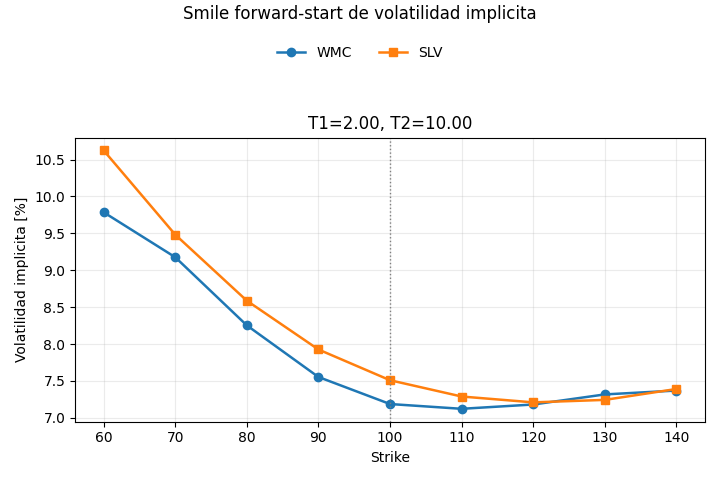
\includegraphics[width=0.75\textwidth]{wmc-slv_forward_start_WLS.png}
\caption{Smile \textit{forward-start} de volatilidad implícita para \(T_1=2\) y \(T_2=10\), obtenido con WMC calibrado por mínimos cuadrados ponderados.}
\label{fig:smile_forward_start_T1_2_T2_10}
\end{figure}

En la Figura \ref{fig:smile_forward_start_T1_2_T2_10} se muestra el smile \textit{forward-start} de volatilidad implícita para el par \((T_1,T_2)=(2,10)\), obtenido mediante WMC con calibración por mínimos cuadrados ponderados. Se observa que la curva generada por WMC reproduce de forma razonable la estructura del smile obtenida bajo Heston--SLV, capturando tanto la curvatura como el mayor nivel de volatilidad implícita para strikes bajos.\medskip

Aunque el ajuste exacto permite obtener precios próximos a los de Heston--SLV en las opciones \textit{forward-start} consideradas, los problemas de estabilidad observados al intentar recuperar la estructura completa del smile indican que esta formulación no resulta suficientemente robusta en este contexto. En cambio, la formulación de mínimos cuadrados ponderados introduce una regularización controlada de las restricciones y permite obtener una estructura de volatilidad implícita más estable.\medskip

Por tanto, los resultados ponen de manifiesto que la proximidad en precios no garantiza necesariamente una buena reproducción de la estructura de volatilidad implícita. En este sentido, el ajuste exacto resulta útil para analizar la aproximación punto a punto de precios, mientras que la formulación de mínimos cuadrados ponderados ofrece un comportamiento más adecuado cuando se estudian instrumentos más sensibles a la dinámica temporal, como las opciones \textit{forward-start}.\medskip

Por su parte, el modelo Heston--SLV incorpora una dinámica estocástica de la volatilidad combinada con una componente local, lo que le permite generar de forma natural una estructura forward de volatilidad más rica. Por ello, las opciones \textit{forward-start} permiten poner de relieve diferencias entre las metodologías que no se aprecian con la misma claridad en la comparación de opciones vanilla.



\chapter{Conclusiones y líneas futuras de investigación}

\section{Conclusiones}

En este trabajo se han estudiado y comparado dos metodologías de valoración de derivados financieros: el modelo de Volatilidad Local Estocástica, en particular Heston--SLV, y el enfoque de Entropía Relativa Mínima implementado mediante \textit{Weighted Monte Carlo}. Ambas metodologías permiten incorporar la información contenida en una superficie de volatilidad implícita, pero lo hacen desde perspectivas diferentes. Mientras que Heston--SLV modifica la dinámica del subyacente combinando una componente local con una componente estocástica de la volatilidad, MRE/WMC mantiene fijas las trayectorias simuladas y ajusta la medida de probabilidad mediante una redistribución de pesos sujeta a restricciones de calibración.\medskip

Los resultados numéricos muestran que, para opciones europeas vanilla, MRE reproduce de forma razonable los precios generados por Heston--SLV, incluso en strikes no utilizados directamente como benchmark. En el caso de las opciones \textit{forward-start}, los precios obtenidos mediante el ajuste exacto también son relativamente próximos a los de Heston--SLV. Sin embargo, el análisis de la volatilidad implícita \textit{forward-start} muestra que la proximidad en precios no garantiza necesariamente una buena reproducción de la estructura de smile forward. En particular, la formulación exacta presenta problemas de estabilidad para capturar dicha estructura, mientras que la formulación regularizada mediante mínimos cuadrados ponderados permite recuperar de forma más adecuada la curvatura del smile. En conjunto, la comparación confirma que ambas metodologías son consistentes para la valoración, pero también pone de manifiesto diferencias relevantes cuando se analizan productos más sensibles a la dinámica temporal del subyacente.


\section{Líneas futuras de investigación}

Como posibles líneas futuras de investigación, una primera extensión de este trabajo consistiría en aplicar ambas metodologías a datos reales de mercado, utilizando superficies de volatilidad implícita observadas para distintos activos y fechas. Esto permitiría analizar con mayor precisión la capacidad de ajuste de los modelos en un contexto más cercano a la práctica financiera.\medskip

Otra línea de trabajo sería ampliar el conjunto de productos derivados considerados. En esta memoria se han valorado principalmente opciones europeas vainilla y opciones de tipo \textit{forward-start}. Sin embargo, sería interesante estudiar el comportamiento de los métodos SLV y MRE/WMC en la valoración de productos más complejos o dependientes de la trayectoria, como opciones asiáticas o barrera.\medskip

También resultaría relevante incorporar un análisis de cobertura. En este trabajo la comparación se ha centrado en los precios obtenidos bajo ambas metodologías, pero una comparación más completa debería estudiar las sensibilidades de los precios frente a los factores de mercado y la estabilidad de las estrategias de cobertura asociadas.\medskip

Finalmente, otra extensión posible sería comparar el enfoque MRE/WMC con variantes más generales, como Generalized Weighted Monte Carlo, o con otros métodos de calibración basados en optimización. Esto permitiría evaluar si una elección distinta de la medida previa o de las restricciones de calibración mejora la estabilidad y precisión de los precios obtenidos.






% ----------------------------------------------------------
%                         Apéndices
% ----------------------------------------------------------
\cleardoublepage
\appendix
% Asegurar que el estilo de página use marcadores (\leftmark/\rightmark)
\pagestyle{headings}
\clearpage
\chapter{Tablas de precios SLV}

\begingroup
\scriptsize
\renewcommand{\arraystretch}{0.82}
\setlength{\tabcolsep}{4pt}
\begin{longtable}{@{}rrrrr@{}}
\caption{Comparación entre precios SLV y precios de mercado para opciones vainilla europeas CALL}\label{tab:slv_vs_bs_call}\\
\toprule
\textbf{Strike} & \textbf{Vencimiento} & \textbf{Precio SLV} & \textbf{Precio mercado} & \textbf{Error absoluto} \\
\midrule
\endfirsthead
\toprule
\textbf{Strike} & \textbf{Vencimiento} & \textbf{Precio SLV} & \textbf{Precio mercado} & \textbf{Error absoluto} \\
\midrule
\endhead
\bottomrule
\endlastfoot
40.00  & 0.02  & 60.00 & 60.00 & 0.00 \\
60.00  & 0.02  & 40.00 & 40.00 & 0.00 \\
80.00  & 0.02  & 20.00 & 20.00 & 0.00 \\
100.00 & 0.02  & 0.42  & 0.28  & 0.14 \\
120.00 & 0.02  & 0.00  & 0.00  & 0.00 \\
140.00 & 0.02  & 0.00  & 0.00  & 0.00 \\
40.00  & 0.08  & 60.00 & 60.00 & 0.00 \\
60.00  & 0.08  & 40.00 & 40.00 & 0.00 \\
80.00  & 0.08  & 20.00 & 20.00 & 0.00 \\
100.00 & 0.08  & 0.78  & 0.58  & 0.20 \\
120.00 & 0.08  & 0.00  & 0.00  & 0.00 \\
140.00 & 0.08  & 0.00  & 0.00  & 0.00 \\
40.00  & 0.50  & 60.03 & 60.00 & 0.03 \\
60.00  & 0.50  & 40.06 & 40.00 & 0.06 \\
80.00  & 0.50  & 20.13 & 20.00 & 0.13 \\
100.00 & 0.50  & 1.79  & 1.56  & 0.23 \\
120.00 & 0.50  & 0.09  & 0.00  & 0.09 \\
140.00 & 0.50  & 0.08  & 0.00  & 0.08 \\
40.00  & 1.00  & 60.06 & 60.00 & 0.06 \\
60.00  & 1.00  & 40.09 & 40.00 & 0.09 \\
80.00  & 1.00  & 20.15 & 20.02 & 0.13 \\
100.00 & 1.00  & 2.55  & 2.41  & 0.14 \\
120.00 & 1.00  & 0.09  & 0.00  & 0.09 \\
140.00 & 1.00  & 0.09  & 0.00  & 0.09 \\
40.00  & 2.00  & 60.07 & 60.00 & 0.07 \\
60.00  & 2.00  & 40.11 & 40.01 & 0.10 \\
80.00  & 2.00  & 20.29 & 20.19 & 0.10 \\
100.00 & 2.00  & 3.64  & 3.49  & 0.15 \\
120.00 & 2.00  & 0.02  & 0.03  & 0.01 \\
140.00 & 2.00  & 0.00  & 0.00  & 0.00 \\
40.00  & 5.00  & 60.12 & 60.05 & 0.07 \\
60.00  & 5.00  & 40.31 & 40.22 & 0.09 \\
80.00  & 5.00  & 21.17 & 21.12 & 0.05 \\
100.00 & 5.00  & 6.06  & 5.92  & 0.14 \\
120.00 & 5.00  & 0.69  & 0.70  & 0.01 \\
140.00 & 5.00  & 0.14  & 0.10  & 0.04 \\
40.00  & 8.00  & 60.16 & 60.11 & 0.05 \\
60.00  & 8.00  & 40.53 & 40.48 & 0.05 \\
80.00  & 8.00  & 22.07 & 22.01 & 0.06 \\
100.00 & 8.00  & 7.99  & 7.90  & 0.09 \\
120.00 & 8.00  & 1.89  & 1.92  & 0.03 \\
140.00 & 8.00  & 0.47  & 0.50  & 0.03 \\
40.00  & 10.00 & 60.18 & 60.12 & 0.06 \\
60.00  & 10.00 & 40.65 & 40.59 & 0.06 \\
80.00  & 10.00 & 22.59 & 22.53 & 0.06 \\
100.00 & 10.00 & 9.15  & 9.09  & 0.06 \\
120.00 & 10.00 & 2.79  & 2.83  & 0.04 \\
140.00 & 10.00 & 0.84  & 0.89  & 0.05 \\
\end{longtable}
\endgroup

\clearpage
\begingroup
\scriptsize
\renewcommand{\arraystretch}{0.82}
\setlength{\tabcolsep}{4pt}
\begin{longtable}{@{}rrrrr@{}}
\caption{Comparación entre precios SLV y precios de mercado Black--Scholes para opciones vainilla europeas PUT}\label{tab:slv_ref_put}\\
\toprule
\textbf{Strike} & \textbf{Vencimiento} & \textbf{Precio SLV} & \textbf{Precio mercado} & \textbf{Error absoluto} \\
\midrule
\endfirsthead
\toprule
\textbf{Strike} & \textbf{Vencimiento} & \textbf{Precio SLV} & \textbf{Precio mercado} & \textbf{Error absoluto} \\
\midrule
\endhead
\bottomrule
\endlastfoot
40.00  & 0.02  & 0.00 & 0.00 & 0.00 \\
60.00  & 0.02  & 0.00 & 0.00 & 0.00 \\
80.00  & 0.02  & 0.00 & 0.00 & 0.00 \\
100.00 & 0.02  & 0.42 & 0.28 & 0.14 \\
120.00 & 0.02  & 20.00 & 20.00 & 0.00 \\
140.00 & 0.02  & 40.00 & 40.00 & 0.00 \\
40.00  & 0.08  & 0.00 & 0.00 & 0.00 \\
60.00  & 0.08  & 0.00 & 0.00 & 0.00 \\
80.00  & 0.08  & 0.00 & 0.00 & 0.00 \\
100.00 & 0.08  & 0.78 & 0.58 & 0.20 \\
120.00 & 0.08  & 20.00 & 20.00 & 0.00 \\
140.00 & 0.08  & 40.00 & 40.00 & 0.00 \\
40.00  & 0.50  & 0.03 & 0.00 & 0.03 \\
60.00  & 0.50  & 0.06 & 0.00 & 0.06 \\
80.00  & 0.50  & 0.13 & 0.00 & 0.13 \\
100.00 & 0.50  & 1.79 & 1.56 & 0.23 \\
120.00 & 0.50  & 20.09 & 20.00 & 0.09 \\
140.00 & 0.50  & 40.08 & 40.00 & 0.08 \\
40.00  & 1.00  & 0.06 & 0.00 & 0.06 \\
60.00  & 1.00  & 0.09 & 0.00 & 0.09 \\
80.00  & 1.00  & 0.15 & 0.02 & 0.13 \\
100.00 & 1.00  & 2.55 & 2.41 & 0.14 \\
120.00 & 1.00  & 20.09 & 20.00 & 0.09 \\
140.00 & 1.00  & 40.09 & 40.00 & 0.09 \\
40.00  & 2.00  & 0.07 & 0.00 & 0.07 \\
60.00  & 2.00  & 0.11 & 0.01 & 0.10 \\
80.00  & 2.00  & 0.29 & 0.19 & 0.10 \\
100.00 & 2.00  & 3.64 & 3.49 & 0.15 \\
120.00 & 2.00  & 20.02 & 20.03 & 0.01 \\
140.00 & 2.00  & 40.00 & 40.00 & 0.00 \\
40.00  & 5.00  & 0.12 & 0.05 & 0.07 \\
60.00  & 5.00  & 0.31 & 0.22 & 0.09 \\
80.00  & 5.00  & 1.17 & 1.12 & 0.05 \\
100.00 & 5.00  & 6.06 & 5.92 & 0.14 \\
120.00 & 5.00  & 20.69 & 20.70 & 0.01 \\
140.00 & 5.00  & 40.14 & 40.10 & 0.04 \\
40.00  & 8.00  & 0.16 & 0.11 & 0.05 \\
60.00  & 8.00  & 0.53 & 0.48 & 0.05 \\
80.00  & 8.00  & 2.07 & 2.01 & 0.06 \\
100.00 & 8.00  & 7.99 & 7.90 & 0.09 \\
120.00 & 8.00  & 21.89 & 21.92 & 0.03 \\
140.00 & 8.00  & 40.47 & 40.50 & 0.03 \\
40.00  & 10.00 & 0.18 & 0.12 & 0.06 \\
60.00  & 10.00 & 0.65 & 0.59 & 0.06 \\
80.00  & 10.00 & 2.59 & 2.53 & 0.06 \\
100.00 & 10.00 & 9.15 & 9.09 & 0.06 \\
120.00 & 10.00 & 22.79 & 22.83 & 0.04 \\
140.00 & 10.00 & 40.84 & 40.89 & 0.05 \\
\end{longtable}
\endgroup

\chapter{Tablas de precios MRE}

\begingroup
\scriptsize
\renewcommand{\arraystretch}{0.82}
\setlength{\tabcolsep}{4pt}
\begin{longtable}{@{}rrrrr@{}}
\caption{Comparación entre precios WMC y precios benchmark para opciones vainilla europeas CALL}\label{tab:wmc_vs_ref_call}\\
\toprule
\textbf{Strike} & \textbf{Vencimiento} & \textbf{Precio WMC} & \textbf{Precio benchmark} & \textbf{Error absoluto} \\
\midrule
\endfirsthead
\toprule
\textbf{Strike} & \textbf{Vencimiento} & \textbf{Precio WMC} & \textbf{Precio benchmark} & \textbf{Error absoluto} \\
\midrule
\endhead
\bottomrule
\endlastfoot
40.00  & 0.02  & 60.00 & 60.00 & 0.00 \\
60.00  & 0.02  & 40.00 & 40.00 & 0.00 \\
80.00  & 0.02  & 20.00 & 20.00 & 0.00 \\
100.00 & 0.02  & 0.42  & 0.42  & 0.00 \\
120.00 & 0.02  & 0.00  & 0.00  & 0.00 \\
140.00 & 0.02  & 0.00  & 0.00  & 0.00 \\
40.00  & 0.08  & 60.00 & 60.00 & 0.00 \\
60.00  & 0.08  & 40.00 & 40.00 & 0.00 \\
80.00  & 0.08  & 20.00 & 20.00 & 0.00 \\
100.00 & 0.08  & 0.78  & 0.78  & 0.00 \\
120.00 & 0.08  & 0.00  & 0.00  & 0.00 \\
140.00 & 0.08  & 0.00  & 0.00  & 0.00 \\
40.00  & 0.50  & 60.00 & 60.03 & 0.03 \\
60.00  & 0.50  & 40.00 & 40.06 & 0.06 \\
80.00  & 0.50  & 20.00 & 20.13 & 0.13 \\
100.00 & 0.50  & 1.79  & 1.79  & 0.00 \\
120.00 & 0.50  & 0.00  & 0.09  & 0.09 \\
140.00 & 0.50  & 0.00  & 0.08  & 0.08 \\
40.00  & 1.00  & 60.00 & 60.06 & 0.06 \\
60.00  & 1.00  & 40.00 & 40.09 & 0.09 \\
80.00  & 1.00  & 20.00 & 20.15 & 0.15 \\
100.00 & 1.00  & 2.55  & 2.55  & 0.00 \\
120.00 & 1.00  & 0.09  & 0.09  & 0.00 \\
140.00 & 1.00  & 0.00  & 0.09  & 0.09 \\
40.00  & 2.00  & 60.00 & 60.07 & 0.07 \\
60.00  & 2.00  & 40.00 & 40.11 & 0.11 \\
80.00  & 2.00  & 20.02 & 20.29 & 0.27 \\
100.00 & 2.00  & 3.64  & 3.64  & 0.00 \\
120.00 & 2.00  & 0.02  & 0.02  & 0.00 \\
140.00 & 2.00  & 0.00  & 0.00  & 0.00 \\
40.00  & 5.00  & 60.00 & 60.12 & 0.12 \\
60.00  & 5.00  & 40.00 & 40.31 & 0.31 \\
80.00  & 5.00  & 20.46 & 21.17 & 0.71 \\
100.00 & 5.00  & 6.06  & 6.06  & 0.00 \\
120.00 & 5.00  & 0.69  & 0.69  & 0.00 \\
140.00 & 5.00  & 0.14  & 0.14  & 0.00 \\
40.00  & 8.00  & 60.00 & 60.16 & 0.16 \\
60.00  & 8.00  & 40.03 & 40.53 & 0.50 \\
80.00  & 8.00  & 21.30 & 22.07 & 0.77 \\
100.00 & 8.00  & 7.99  & 7.99  & 0.00 \\
120.00 & 8.00  & 1.89  & 1.89  & 0.00 \\
140.00 & 8.00  & 0.47  & 0.47  & 0.00 \\
40.00  & 10.00 & 60.00 & 60.18 & 0.18 \\
60.00  & 10.00 & 40.09 & 40.65 & 0.56 \\
80.00  & 10.00 & 21.93 & 22.59 & 0.66 \\
100.00 & 10.00 & 9.15  & 9.15  & 0.00 \\
120.00 & 10.00 & 2.79  & 2.79  & 0.00 \\
140.00 & 10.00 & 0.84  & 0.84  & 0.00 \\
\end{longtable}
\endgroup

\clearpage
\begingroup
\scriptsize
\renewcommand{\arraystretch}{0.82}
\setlength{\tabcolsep}{4pt}
\begin{longtable}{@{}rrrrr@{}}
\caption{Comparación entre precios WMC y precios benchmark para opciones vainilla europeas PUT}\label{tab:wmc_vs_ref_put}\\
\toprule
\textbf{Strike} & \textbf{Vencimiento} & \textbf{Precio WMC} & \textbf{Precio benchmark} & \textbf{Error absoluto} \\
\midrule
\endfirsthead
\toprule
\textbf{Strike} & \textbf{Vencimiento} & \textbf{Precio WMC} & \textbf{Precio benchmark} & \textbf{Error absoluto} \\
\midrule
\endhead
\bottomrule
\endlastfoot
40.00  & 0.02  & 0.00 & 0.00 & 0.00 \\
60.00  & 0.02  & 0.00 & 0.00 & 0.00 \\
80.00  & 0.02  & 0.00 & 0.00 & 0.00 \\
100.00 & 0.02  & 0.42 & 0.42 & 0.00 \\
120.00 & 0.02  & 20.00 & 20.00 & 0.00 \\
140.00 & 0.02  & 40.00 & 40.00 & 0.00 \\
40.00  & 0.08  & 0.00 & 0.00 & 0.00 \\
60.00  & 0.08  & 0.00 & 0.00 & 0.00 \\
80.00  & 0.08  & 0.00 & 0.00 & 0.00 \\
100.00 & 0.08  & 0.78 & 0.78 & 0.00 \\
120.00 & 0.08  & 20.00 & 20.00 & 0.00 \\
140.00 & 0.08  & 40.00 & 40.00 & 0.00 \\
40.00  & 0.50  & 0.00 & 0.00 & 0.00 \\
60.00  & 0.50  & 0.00 & 0.00 & 0.00 \\
80.00  & 0.50  & 0.00 & 0.00 & 0.00 \\
100.00 & 0.50  & 1.79 & 1.79 & 0.00 \\
120.00 & 0.50  & 20.00 & 20.00 & 0.00 \\
140.00 & 0.50  & 40.00 & 40.00 & 0.00 \\
40.00  & 1.00  & 0.00 & 0.00 & 0.00 \\
60.00  & 1.00  & 0.00 & 0.00 & 0.00 \\
80.00  & 1.00  & 0.00 & 0.00 & 0.00 \\
100.00 & 1.00  & 2.55 & 2.55 & 0.00 \\
120.00 & 1.00  & 20.09 & 20.09 & 0.00 \\
140.00 & 1.00  & 40.00 & 40.00 & 0.00 \\
40.00  & 2.00  & 0.00 & 0.00 & 0.00 \\
60.00  & 2.00  & 0.00 & 0.00 & 0.00 \\
80.00  & 2.00  & 0.02 & 0.02 & 0.00 \\
100.00 & 2.00  & 3.64 & 3.64 & 0.00 \\
120.00 & 2.00  & 20.02 & 20.02 & 0.00 \\
140.00 & 2.00  & 40.00 & 40.00 & 0.00 \\
40.00  & 5.00  & 0.00 & 0.00 & 0.00 \\
60.00  & 5.00  & 0.00 & 0.00 & 0.00 \\
80.00  & 5.00  & 0.46 & 0.46 & 0.00 \\
100.00 & 5.00  & 6.06 & 6.06 & 0.00 \\
120.00 & 5.00  & 20.69 & 20.69 & 0.00 \\
140.00 & 5.00  & 40.14 & 40.14 & 0.00 \\
40.00  & 8.00  & 0.00 & 0.00 & 0.00 \\
60.00  & 8.00  & 0.03 & 0.03 & 0.00 \\
80.00  & 8.00  & 1.30 & 1.30 & 0.00 \\
100.00 & 8.00  & 7.99 & 7.99 & 0.00 \\
120.00 & 8.00  & 21.89 & 21.89 & 0.00 \\
140.00 & 8.00  & 40.47 & 40.47 & 0.00 \\
40.00  & 10.00 & 0.00 & 0.00 & 0.00 \\
60.00  & 10.00 & 0.09 & 0.09 & 0.00 \\
80.00  & 10.00 & 1.93 & 1.93 & 0.00 \\
100.00 & 10.00 & 9.15 & 9.15 & 0.00 \\
120.00 & 10.00 & 22.79 & 22.79 & 0.00 \\
140.00 & 10.00 & 40.84 & 40.84 & 0.00 \\
\end{longtable}
\endgroup

\chapter{Resultados para opciones forward-start}

\section{Valoración bajo el modelo Heston--SLV}

\begin{table}[H]
\centering
\caption{Resultados completos de valoración de opciones forward-start bajo Heston--SLV.}
\label{tab:apendice_forward_slv}
\scriptsize
\renewcommand{\arraystretch}{0.84}
\begin{tabular}{@{}rrrrr@{}}
\toprule
\textbf{Strike} & \textbf{\(T_1\)} & \textbf{\(T_2\)} & \textbf{Precio SLV (Call)} & \textbf{Precio SLV (Put)} \\
\midrule
70.00  & 0.50 & 1.00  & 30.05 & 0.05  \\
90.00  & 0.50 & 1.00  & 10.16 & 0.16  \\
110.00 & 0.50 & 1.00  & 0.12  & 10.12 \\
70.00  & 0.50 & 2.00  & 30.09 & 0.09  \\
90.00  & 0.50 & 2.00  & 10.71 & 0.71  \\
110.00 & 0.50 & 2.00  & 0.29  & 10.29 \\
70.00  & 0.50 & 5.00  & 30.48 & 0.48  \\
90.00  & 0.50 & 5.00  & 12.49 & 2.49  \\
110.00 & 0.50 & 5.00  & 2.09  & 12.09 \\
70.00  & 0.50 & 10.00 & 31.20 & 1.20  \\
90.00  & 0.50 & 10.00 & 14.90 & 4.90  \\
110.00 & 0.50 & 10.00 & 5.06  & 15.06 \\
70.00  & 1.00 & 2.00  & 30.09 & 0.09  \\
90.00  & 1.00 & 2.00  & 10.50 & 0.50  \\
110.00 & 1.00 & 2.00  & 0.12  & 10.12 \\
70.00  & 1.00 & 5.00  & 30.45 & 0.45  \\
90.00  & 1.00 & 5.00  & 12.33 & 2.33  \\
110.00 & 1.00 & 5.00  & 1.84  & 11.84 \\
70.00  & 1.00 & 10.00 & 31.16 & 1.16  \\
90.00  & 1.00 & 10.00 & 14.77 & 4.77  \\
110.00 & 1.00 & 10.00 & 4.90  & 14.90 \\
70.00  & 2.00 & 5.00  & 30.27 & 0.27  \\
90.00  & 2.00 & 5.00  & 11.82 & 1.82  \\
110.00 & 2.00 & 5.00  & 1.29  & 11.29 \\
70.00  & 2.00 & 10.00 & 30.95 & 0.95  \\
90.00  & 2.00 & 10.00 & 14.39 & 4.39  \\
110.00 & 2.00 & 10.00 & 4.52  & 14.52 \\
70.00  & 5.00 & 10.00 & 30.46 & 0.46  \\
90.00  & 5.00 & 10.00 & 13.13 & 3.13  \\
110.00 & 5.00 & 10.00 & 3.03  & 13.03 \\
\bottomrule
\end{tabular}
\end{table}

\section{Valoración mediante Entropía Relativa Mínima}

\begin{table}[H]
\centering
\caption{Resultados completos de valoración de opciones forward-start bajo Entropía relativa.}
\label{tab:forward_start_mre}
\scriptsize
\renewcommand{\arraystretch}{0.84}
\begin{tabular}{@{}rrrrr@{}}
\toprule
\textbf{Strike} & \textbf{\(T_1\)} & \textbf{\(T_2\)} & \textbf{Precio WMC (Call)} & \textbf{Precio WMC (Put)} \\
\midrule
70.00  & 0.50 & 1.00  & 30.00 & 0.00  \\
90.00  & 0.50 & 1.00  & 10.02 & 0.02  \\
110.00 & 0.50 & 1.00  & 0.08  & 10.08 \\
70.00  & 0.50 & 2.00  & 30.00 & 0.00  \\
90.00  & 0.50 & 2.00  & 10.34 & 0.34  \\
110.00 & 0.50 & 2.00  & 0.42  & 10.42 \\
70.00  & 0.50 & 5.00  & 30.03 & 0.03  \\
90.00  & 0.50 & 5.00  & 11.94 & 1.94  \\
110.00 & 0.50 & 5.00  & 2.07  & 12.07 \\
70.00  & 0.50 & 10.00 & 30.50 & 0.50  \\
90.00  & 0.50 & 10.00 & 14.54 & 4.54  \\
110.00 & 0.50 & 10.00 & 5.13  & 15.13 \\
70.00  & 1.00 & 2.00  & 30.00 & 0.00  \\
90.00  & 1.00 & 2.00  & 10.12 & 0.12  \\
110.00 & 1.00 & 2.00  & 0.16  & 10.16 \\
70.00  & 1.00 & 5.00  & 30.02 & 0.02  \\
90.00  & 1.00 & 5.00  & 11.67 & 1.67  \\
110.00 & 1.00 & 5.00  & 1.75  & 11.75 \\
70.00  & 1.00 & 10.00 & 30.43 & 0.43  \\
90.00  & 1.00 & 10.00 & 14.36 & 4.36  \\
110.00 & 1.00 & 10.00 & 4.89  & 14.89 \\
70.00  & 2.00 & 5.00  & 30.00 & 0.00  \\
90.00  & 2.00 & 5.00  & 11.26 & 1.26  \\
110.00 & 2.00 & 5.00  & 1.48  & 11.48 \\
70.00  & 2.00 & 10.00 & 30.36 & 0.36  \\
90.00  & 2.00 & 10.00 & 14.04 & 4.04  \\
110.00 & 2.00 & 10.00 & 4.66  & 14.66 \\
70.00  & 5.00 & 10.00 & 30.11 & 0.11  \\
90.00  & 5.00 & 10.00 & 12.74 & 2.74  \\
110.00 & 5.00 & 10.00 & 3.21  & 13.21 \\
\bottomrule
\end{tabular}
\end{table}



% % % % % % % % % % % % % % % % % % % % % % % % % % % % % % % % % % % % %
%                          Bibliografia                                 %
% % % % % % % % % % % % % % % % % % % % % % % % % % % % % % % % % % % % %
\nocite{*} %Imprime todas las entradas del .bib aunque no estén citadas
\bibliography{referencias}



\end{document}
% % % % % % % % % % % % % % % % % % % % % % % % % % % % % % % % % % % % %
% % % % % % % % % % % % % % % % % % % % % % % % % % % % % % % % % % % % % 
